%%% Hlavní soubor. Zde se definují základní parametry a odkazuje se na ostatní části. %%%

%% Verze pro jednostranný tisk:
% Okraje: levý 40mm, pravý 25mm, horní a dolní 25mm
% (ale pozor, LaTeX si sám přidává 1in)
\documentclass[12pt,a4paper]{report}
\setlength\textwidth{145mm}
\setlength\textheight{247mm}
\setlength\oddsidemargin{15mm}
\setlength\evensidemargin{15mm}
\setlength\topmargin{0mm}
\setlength\headsep{0mm}
\setlength\headheight{0mm}
% \openright zařídí, aby následující text začínal na pravé straně knihy
\let\openright=\clearpage

%% Pokud tiskneme oboustranně:
% \documentclass[12pt,a4paper,twoside,openright]{report}
% \setlength\textwidth{145mm}
% \setlength\textheight{247mm}
% \setlength\oddsidemargin{14.2mm}
% \setlength\evensidemargin{0mm}
% \setlength\topmargin{0mm}
% \setlength\headsep{0mm}
% \setlength\headheight{0mm}
% \let\openright=\cleardoublepage

%% Vytváříme PDF/A-2u
\usepackage[a-2u]{pdfx}

%% Přepneme na českou sazbu a fonty Latin Modern
\usepackage[czech]{babel}
\usepackage{lmodern}
\usepackage[T1]{fontenc}
\usepackage{textcomp}

%% Použité kódování znaků: obvykle latin2, cp1250 nebo utf8:
\usepackage[utf8]{inputenc}

%%% Další užitečné balíčky (jsou součástí běžných distribucí LaTeXu)
\usepackage{amsmath}        % rozšíření pro sazbu matematiky
\usepackage{amsfonts}       % matematické fonty
\usepackage{amsthm}         % sazba vět, definic apod.
\usepackage{bbding}         % balíček s nejrůznějšími symboly
			    % (čtverečky, hvězdičky, tužtičky, nůžtičky, ...)
\usepackage{bm}             % tučné symboly (příkaz \bm)
\usepackage{graphicx}       % vkládání obrázků
\usepackage{fancyvrb}       % vylepšené prostředí pro strojové písmo
\usepackage{indentfirst}    % zavede odsazení 1. odstavce kapitoly
\usepackage{natbib}         % zajištuje možnost odkazovat na literaturu
			    % stylem AUTOR (ROK), resp. AUTOR [ČÍSLO]
\usepackage[nottoc]{tocbibind} % zajistí přidání seznamu literatury,
                            % obrázků a tabulek do obsahu
\usepackage{icomma}         % inteligetní čárka v matematickém módu
\usepackage{dcolumn}        % lepší zarovnání sloupců v tabulkách
\usepackage{booktabs}       % lepší vodorovné linky v tabulkách
\usepackage{paralist}       % lepší enumerate a itemize
\usepackage{xcolor}         % barevná sazba

%%% Údaje o práci

% Název práce v jazyce práce (přesně podle zadání)
\def\NazevPrace{ServIS – webový systém pro firmy zabývající se opravami bagrů}

% Název práce v angličtině
\def\NazevPraceEN{ServIS – a web system for companies dealing with excavator repairs}

% Jméno autora
\def\AutorPrace{Milan Truchan}

% Rok odevzdání
\def\RokOdevzdani{2023}

% Název katedry nebo ústavu, kde byla práce oficiálně zadána
% (dle Organizační struktury MFF UK, případně plný název pracoviště mimo MFF)
\def\Katedra{Katedra distribuovaných a spolehlivých systémů}
\def\KatedraEN{Department of Distributed and Dependable Systems}

% Jedná se o katedru (department) nebo o ústav (institute)?
\def\TypPracoviste{Katedra}
\def\TypPracovisteEN{Department}

% Vedoucí práce: Jméno a příjmení s~tituly
\def\Vedouci{Mgr. Pavel Ježek, Ph.D.}

% Pracoviště vedoucího (opět dle Organizační struktury MFF)
\def\KatedraVedouciho{Katedra distribuovaných a spolehlivých systémů}
\def\KatedraVedoucihoEN{Department of Distributed and Dependable Systems}

% Studijní program a obor
\def\StudijniProgram{Informatika}
\def\StudijniObor{Programování a vývoj software}

% Nepovinné poděkování (vedoucímu práce, konzultantovi, tomu, kdo
% zapůjčil software, literaturu apod.)
\def\Podekovani{%
Poděkování.
}

% Abstrakt (doporučený rozsah cca 80-200 slov; nejedná se o zadání práce)
\def\Abstrakt{%
Cieľom tejto práce bolo vytvoriť softvérové dielo pre malé firmy\\ zaoberajúce sa zemnými a výkopovými prácami, opravou a predajom bagrov, ktoré nemajú prístup k vhodnému softvérovému riešeniu pre svoju činnosť.

Potreba a správanie funkcionalít bola prekonzultovaná s majiteľom jednej z týchto firiem.

Vzniknutý softvér predstavuje riešenie problému, je schopný zobraziť ponuku (stroje, prídavné zariadenia) a umožňuje užívateľom dopyt (v podobe emailov) na tieto ponuky. V aplikácii tiež existuje aukcia, kde sa dražia opravené bagre. Užívatelia si tiež môžu v aplikácií vytvoriť účet. Vymenované funkcionality môžu využívať prihlásení aj neprihlásení užívatelia. Bežní prihlásení užívatelia nemusia vyplňovať informácie o sebe vo formulároch pri dopytovaní sa na ponuku. Prihlásení admini majú možnosť spravovať stránku. Tj. pridávať nové, editovať a mazať existujúce ponuky, odpovedať na správy atď.

}
\def\AbstraktEN{%
Abstract.
}

% 3 až 5 klíčových slov (doporučeno), každé uzavřeno ve složených závorkách
\def\KlicovaSlova{%
{Informačný systém} {C\#} {.NET} {Blazor Server} {MySQL}
}
\def\KlicovaSlovaEN{%
{Information system} {C\#} {.NET} {Blazor Server} {MySQL}
}

%% Balíček hyperref, kterým jdou vyrábět klikací odkazy v PDF,
%% ale hlavně ho používáme k uložení metadat do PDF (včetně obsahu).
%% Většinu nastavítek přednastaví balíček pdfx.
\hypersetup{unicode}
\hypersetup{breaklinks=true}

%% Definice různých užitečných maker (viz popis uvnitř souboru)
%%% Tento soubor obsahuje definice různých užitečných maker a prostředí %%%
%%% Další makra připisujte sem, ať nepřekáží v ostatních souborech.     %%%

%%% Drobné úpravy stylu

% Tato makra přesvědčují mírně ošklivým trikem LaTeX, aby hlavičky kapitol
% sázel příčetněji a nevynechával nad nimi spoustu místa. Směle ignorujte.
\makeatletter
\def\@makechapterhead#1{
  {\parindent \z@ \raggedright \normalfont
   \Huge\bfseries \thechapter. #1
   \par\nobreak
   \vskip 20\p@
}}
\def\@makeschapterhead#1{
  {\parindent \z@ \raggedright \normalfont
   \Huge\bfseries #1
   \par\nobreak
   \vskip 20\p@
}}
\makeatother

% Toto makro definuje kapitolu, která není očíslovaná, ale je uvedena v obsahu.
\def\chapwithtoc#1{
\chapter*{#1}
\addcontentsline{toc}{chapter}{#1}
}

% Trochu volnější nastavení dělení slov, než je default.
\lefthyphenmin=2
\righthyphenmin=2

% Zapne černé "slimáky" na koncích řádků, které přetekly, abychom si
% jich lépe všimli.
\overfullrule=1mm

%%% Makra pro definice, věty, tvrzení, příklady, ... (vyžaduje baliček amsthm)

\theoremstyle{plain}
\newtheorem{veta}{Věta}
\newtheorem{lemma}[veta]{Lemma}
\newtheorem{tvrz}[veta]{Tvrzení}

\theoremstyle{plain}
\newtheorem{definice}{Definice}

\theoremstyle{remark}
\newtheorem*{dusl}{Důsledek}
\newtheorem*{pozn}{Poznámka}
\newtheorem*{prikl}{Příklad}

%%% Prostředí pro důkazy

\newenvironment{dukaz}{
  \par\medskip\noindent
  \textit{Důkaz}.
}{
\newline
\rightline{$\qedsymbol$}
}

%%% Prostředí pro sazbu kódu, případně vstupu/výstupu počítačových
%%% programů. (Vyžaduje balíček fancyvrb -- fancy verbatim.)

\DefineVerbatimEnvironment{code}{Verbatim}{fontsize=\small, frame=single}

%%% Prostor reálných, resp. přirozených čísel
\newcommand{\R}{\mathbb{R}}
\newcommand{\N}{\mathbb{N}}

%%% Užitečné operátory pro statistiku a pravděpodobnost
\DeclareMathOperator{\pr}{\textsf{P}}
\DeclareMathOperator{\E}{\textsf{E}\,}
\DeclareMathOperator{\var}{\textrm{var}}
\DeclareMathOperator{\sd}{\textrm{sd}}

%%% Příkaz pro transpozici vektoru/matice
\newcommand{\T}[1]{#1^\top}

%%% Vychytávky pro matematiku
\newcommand{\goto}{\rightarrow}
\newcommand{\gotop}{\stackrel{P}{\longrightarrow}}
\newcommand{\maon}[1]{o(n^{#1})}
\newcommand{\abs}[1]{\left|{#1}\right|}
\newcommand{\dint}{\int_0^\tau\!\!\int_0^\tau}
\newcommand{\isqr}[1]{\frac{1}{\sqrt{#1}}}

%%% Vychytávky pro tabulky
\newcommand{\pulrad}[1]{\raisebox{1.5ex}[0pt]{#1}}
\newcommand{\mc}[1]{\multicolumn{1}{c}{#1}}


%% Titulní strana a různé povinné informační strany
\begin{document}
%%% Titulní strana práce a další povinné informační strany

%%% Titulní strana práce

\pagestyle{empty}
\hypersetup{pageanchor=false}

\begin{center}

\centerline{\mbox{
\includegraphics[width=166mm]{../img/logo-cs.pdf}}}

\vspace{-8mm}
\vfill

{\bf\Large BAKALÁŘSKÁ PRÁCE}

\vfill

{\LARGE\AutorPrace}

\vspace{15mm}

{\LARGE\bfseries\NazevPrace}

\vfill

\Katedra

\vfill

{
\centerline{\vbox{\halign{\hbox to 0.45\hsize{\hfil #}&\hskip 0.5em\parbox[t]{0.45\hsize}{\raggedright #}\cr
Vedoucí bakalářské práce:&\Vedouci \cr
\noalign{\vspace{2mm}}
Studijní program:&\StudijniProgram \cr
\noalign{\vspace{2mm}}
Studijní obor:&\StudijniObor \cr
}}}}

\vfill

% Zde doplňte rok
Praha \RokOdevzdani

\end{center}

\newpage

%%% Následuje vevázaný list -- kopie podepsaného "Zadání bakalářské práce".
%%% Toto zadání NENÍ součástí elektronické verze práce, nescanovat.

%%% Strana s čestným prohlášením k bakalářské práci

\openright
\hypersetup{pageanchor=true}
\pagestyle{plain}
\pagenumbering{roman}
\vglue 0pt plus 1fill

\noindent
Prohlašuji, že jsem tuto bakalářskou práci vypracoval(a) samostatně a výhradně
s~použitím citovaných pramenů, literatury a dalších odborných zdrojů.
Tato práce nebyla využita k získání jiného nebo stejného titulu.

\medskip\noindent
Beru na~vědomí, že se na moji práci vztahují práva a povinnosti vyplývající
ze zákona č. 121/2000 Sb., autorského zákona v~platném znění, zejména skutečnost,
že Univerzita Karlova má právo na~uzavření licenční smlouvy o~užití této
práce jako školního díla podle §60 odst. 1 autorského zákona.

\vspace{10mm}

\hbox{\hbox to 0.5\hsize{%
V \hbox to 6em{\dotfill} dne \hbox to 6em{\dotfill}
\hss}\hbox to 0.5\hsize{\dotfill\quad}}
\smallskip
\hbox{\hbox to 0.5\hsize{}\hbox to 0.5\hsize{\hfil Podpis autora\hfil}}

\vspace{20mm}
\newpage

%%% Poděkování

\openright

\noindent
\Podekovani

\newpage

%%% Povinná informační strana bakalářské práce

\openright

\vbox to 0.5\vsize{
\setlength\parindent{0mm}
\setlength\parskip{5mm}

Název práce:
\NazevPrace

Autor:
\AutorPrace

\TypPracoviste:
\Katedra

Vedoucí bakalářské práce:
\Vedouci, \KatedraVedouciho

Abstrakt:
\Abstrakt

Klíčová slova:
\KlicovaSlova

\vss}
\newpage \openright %\nobreak
\vbox to 0.49\vsize{
\setlength\parindent{0mm}
\setlength\parskip{5mm}

Title:
\NazevPraceEN

Author:
\AutorPrace

\TypPracovisteEN:
\KatedraEN

Supervisor:
\Vedouci, \KatedraVedoucihoEN

Abstract:
\AbstraktEN

Keywords:
\KlicovaSlovaEN

\vss}

\newpage

\openright
\pagestyle{plain}
\pagenumbering{arabic}
\setcounter{page}{1}


%%% Strana s automaticky generovaným obsahem bakalářské práce

\tableofcontents

%%% Jednotlivé kapitoly práce jsou pro přehlednost uloženy v samostatných souborech
\chapter{Úvod}

V~súčasnosti existujú malé firmy, ktoré fungujú ako dodávatelia rôznych drahých produktov. Tieto firmy môžu ponúkať na~predaj okrem nových produktov aj staré produkty, ktoré prešli nejakou opravou. Takisto stojí za~zmienku, že kedže ide o~dodávateľov drahých produktov, tak zákazníci sa najprv s~firmou musia dohodnúť na~detailoch obchodu, a~až potom je možné dodanie produktu.

Spoločným problémom takýchto firiem býva, že ich ľudia nepoznajú. Preto by sa spomínaným firmám hodilo riešenie, ktoré by im umožnilo zviditeľniť ich ponuku produktov. Jednoduché riešenie v~podobe statických stránok v~tomto prípade nestačí, pretože by neumožnilo dynamicky meniť ponuku danej firmy. Použitie nejakého CMS systému~(z~ang. content management system), napr.~Word\-Press, takisto nie je optimálnym riešením, pretože vyžaduje znalosť platformy, ktorá nie je samozrejmesťou.

My sme dostali ponuku na~tvorbu riešenia od~jednej z~takýchto firiem. Konkrétne ide o~firmu, ktorá sa zaoberá predajom a~opravou bagrov (ďalej už len klientská firma). Po~konzultácii s~majiteľom (ďalej už len klient) sme zistili, že\linebreak klientská firma ponúka služby v~podobe výkopových prác, predaja a~opravy ba\-grov, a~takisto predaja prídavných zariadení pre~bagre. Taktiež sme zistili, že doteraz fungovala komunikácia medzi klientskou firmou a~zákazníkmi prostredníctvom telefonátov, emailov alebo sa strany fyzicky stretli a~dohodli obchod. Klient od~nás vyžaduje riešenie, ktoré by spĺňalo požiadavky uvedené v~následujúcej podkapitole.

\section{Požiadavky na systém}
\label{poziadavky}

V priebehu niekoľkých stretnutí sme s~klientom prebrali a~vypracovali následujúce požiadavky, ktoré musí softvér spĺňať:

\begin{itemize}
\item \textbf{P1 Roly užívateľa}
\label{roly uzivatela}

Jednou z~požiadaviek je, že softvér má rozlišovať zamestnancov firmy spravujúcich systém (ďalej už len administrátori, resp.~administrátor) a~bežných zákazníkov. Obom rolám sa bude zobrazovať len obsah podľa funkcionalít, ktoré majú k~dispozícii. Čiže napr.~zákazník si bude môcť zobraziť detail bagra a~vyjadriť oň nejakým spôsobom záujem, ale nezobrazí sa mu možnosť na~jeho vymazanie. V~prípade administrátora bude možné bager napr.~vymazať, ale nedáva zmysel, aby mohol administrátor vyjadrovať záujem o~bager.

\item \textbf{P2 Predstavenie ponuky zákazníkom}

Ako už bolo spomenuté, klientská firma predáva bagre a~prídavné zariadenia pre~bagre. Klient preto chce, aby bol softvér schopný prezentovať ponuku firmy (bagre a~prídavné zariadenia), pričom hlavná ponuka je tvorená bagrami. Klient vyžaduje, aby po~príchode užívateľa na~domovskú (úvodnú) stránku sa zobrazila hlavná ponuka.
\newpage
\begin{itemize}
\item \textbf{P2.1 Hlavná ponuka}

Hlavná ponuka predstavuje bagre určitého typu (t.~j.~určitej kombinácie značky a~kategórie). Hlavná ponuka obsahuje opis typu bagrov a~fotku reprezentujúcu daný typ bagrov. Všetky tieto údaje okrem opisu sú povinné. Po~rozkliknutí nejakej hlavnej ponuky sa zobrazia bagre typu asociovaného s~vybranou ponukou.

\item \textbf{P2.2 Bager}

Každý bager má obsahovať informácie: názov, značku, kategóriu, opis, fotky a~vlastnosti, pričom všetky okrem opisu sú povinné. Vlastnosti bagra sú určené kombináciou jeho značky a~kategórie (teda typom bagra, každý typ bagra môže mať rôzne vlastnosti, napr. jeden typ bagra by mohol mať vlastnosť ťažná sila, iný typ bagra by mohol mať vlasnosť šírka lyžice). Informácie o~bagri majú byť viditeľné pre~každého užívateľa, t.~j.~ako pre~bežného zákazníka, tak aj\linebreak pre~administrátora. Navyše má ešte stroj obsahovať informáciu o~náhradných dieloch~-- táto informácia má byť viditeľná iba\linebreak pre~administrátorov. Taktiež platí, že môžu existovať bagre, ktoré nepatria do~ponuky a~môžu byť využité výhradne iba v~aukcii (viac o~aukcii v~P4).

\item \textbf{P2.3 Prídavné zariadenie}

Každé prídavné zariadenie má obsahovať informácie: názov, značka, kategória, pre~akú kategóriu bagrov je prídavné zariadenie určené, opis a~fotky, pričom všetky okrem opisu sú povinné. Tieto informácie majú byť viditeľné rovnako pre~každého užívateľa.

\item \textbf{P2.4 Správa bagrov, prídavných zariadení a hlavných ponúk}

Aby mohol administrátor spravovať bagre, prídavné zariadenia,\linebreak ale~takisto aj hlavné ponuky podľa potreby, tak je tiež nutné vytvoriť miesto, ktoré mu ich systém umožní pridávať, odstraňovať a~editovať.
\end{itemize}

\item \textbf{P3 Posielanie dopytu}

Takisto klient od~softvéru vyžaduje, aby umožnil zákazníkom objednať si daný produkt alebo službu prostredníctvom emailových správ. Bežnou\linebreak praxou v~tomto odvetví je, že cena strojov sa dopredu neudáva. Zákazník najprv vyjadrí záujem (dopyt), prekonzultujú sa detaily medzi potenciálnym kupcom a~firmou, a~až potom prebehne obchod. Z~tohto dôvodu systém nebude fungovať na~princípe ako bežné internetové obchody (tým sa myslí pridávanie do~košíka s~následnou platbou), ale bude fungovať na~princípe posielania správ~(dopytov).

\begin{itemize}
\item \textbf{P3.1 Dopyt}

Dopyt by mal v~sebe obsahovať informácie o~žiadanom predmete, údaje o~užívateľovi, a~tiež správu užívateľa. Užívateľskými údajmi sa myslí meno, priezvisko, email~-- tie sú povinné údaje. A~takisto telefónne číslo, mesto~-- tie sú nepovinné údaje.
\end{itemize}
\newpage
\item \textbf{P4 Aukcia}

Keď sme v~predošlých podmienkách spomínali ponuku strojov a~prídavných zariadení, tak išlo o~nové produkty. No ako už bolo skôr spomenuté, klientská firma sa špecializuje aj na~opravu bagrov.

Klient vyžaduje, aby mohol administrátor v~systéme vytvoriť aukčnú ponuku, ktorej môže špecifikovať dátum jej konca, pričom administrátor nesmie byť schopný nastaviť túto hodnotu do~minulosti, počiatočnú sumu (vyvolávaciu cenu), ktorá nesmie byť záporná, popis ponuky (v~popise môže napísať napr.~čo bolo v~bagri opravované), a~takisto aby mohol do ponuky vybrať (opravený) bager. Všetky tieto údaje okrem popisu sú povinné.

Ďalej klient vyžaduje aby systém umožnil zákazníkom ponúkať sumy (prvá ponúknutá suma môže byť rovná počiatočnej sume, nasledujúce ponúkané sumy musia mať medzi sebou rozdiel aspoň 100 eur), pričom po~skončení dražby zákazník s~najvyššou ponúknutou sumou vyhráva dražený bager.

\begin{itemize}
\item \textbf{P4.1 Správanie aukcie}

Keď aukcia skončí, systém má upozorniť jej účastníkov (poslať email s~automaticky generovanou správou) na~to, či vyhrali alebo prehrali dražbu. Taktiež má softvér upozorniť administrátora systému na~to, že aukcia skončila a~kto je jej víťazom. V~prípade, že aukcia skončila bez~víťaza (nikto sa jej nezúčastnil), tak stále platí, že má na~to softvér administrátora upozorniť, ale~taktiež má dražbu automaticky reštartovať, posunúť termín konca dražby o~týždeň a~upozorniť o~tom administrátora (poslať mu email).

\item \textbf{P4.2 Odpočet a ďalšie údaje}

Okrem toho sa od~nášho softvéru vyžaduje, aby bol pri~každej aukčnej ponuke zobrazený odpočet do~konca danej dražby, počet účastníkov, a~taktiež aktuálna (najvyššia ponúknutá) suma.
\end{itemize}

\item \textbf{P5 Správy}

Keďže posielanie dopytov a~správanie aukcie zahŕňa posielanie emailov administrátorom, tak je tiež žiadúce, aby sa emaily dali prečítať nielen z~Gmailu (emailová služba používaná klientom), ale aj z~nášho systému a~rovnako aby systém administrátorom umožnil na~ne odpovedať.

\begin{itemize}
\item \textbf{P5.1 Podobnosť s~Gmailom}

Nakoľko je klient zvyknutý na~prácu s~Gmailom, tak sa má schránka podobať na~Gmail. Teda aspoň funkcionalitou, t.~j.~pri~príchode do~schránky sa zobrazia najnovšie správy pre~každú konverzáciu (vlákno) zoradené zhora smerom dole od~najnovšej po~najstaršiu.

Po~rozkliknutí nejakej zo~správ sa zobrazí celá konverzácia (každá správa vo~vybranom vlákne) zoradená zhora dole od~najstaršej po~najnovšiu.

Ďalej má schránka umožňovať označovanie správ, pričom označené správy budeme môcť hromadne vymazať alebo označiť za~prečítané, resp.~neprečítané. Ak sú označené správy neprečítané, zobrazí sa tlačidlo umožňujúce označenie vybraných správ ako prečítané, ak sú všetky označené správy prečítané, tak sa zobrazí tlačidlo umožňujúce označiť vybrané správy ako neprečítané, a~ak označené správy obsahujú aj prečítané, aj neprečítané správy, tak sa zobrazí tlačidlo umožňujúce označiť vybrané správy ako prečítané.

Podobne po~rozkliknutí nejakej zo~správ sa nám zobrazí celá konverzácia a~administrátor bude môcť celú konverzáciu vymazať alebo~označiť za~neprečítanú, a~taktiež bude môcť odoslať novú správu do~konverzácie (odpovedať na~správy). 

Čo sa týka mazania správ, tak po~kliknutí na~tlačidlo vymazania správy (resp.~správ) stačí ak sa zobrazí potvrdzovacie okno, nie je nutné vytvárať osobitné miesto pre~vymazané správy (kôš). 

\item \textbf{P5.2 Prepojenie správy s~predmetom}

Okrem toho budeme ešte od~softvéru vyžadovať, aby v~správach, ktoré boli odoslané z~nášho systému, ako napr.~dopyt alebo~správy z~aukcie, tak aby v~sebe obsahovali okno, ktoré prepojí správu a~vec, ktorej sa daná správa týka. Teda napríklad ak zákazník odošle dopyt na~stroj~X, tak po~otvorení správy nájde administrátor okrem predmetu a~tela správy, takisto nejaký odkaz (prepojenie) odkazujúci na~stroj~X, ktorým sa dá jednoducho dostať k~údajom o~stroji~X.

\item \textbf{P5.3 Automaticky generované správy}

Okrem toho je tiež žiadúce, aby systém umožnil administrátorom upravovať formát automaticky generovaných (odosielaných) správ týkajúcich sa aukcie.
\end{itemize}

\item \textbf{P6 Registrácia a~prihlásenie užívateľov}

Ďalšou požiadavkou je, aby softvér umožnil zákazníkom registrovať sa do~systému a~následne sa doň prihlásiť. Do~systému sa môžu prihlasovať rovnakým spôsobom ako bežní zákazníci aj administrátori. Systém má rozlíšiť, či ide o~účet bežného zákazníka alebo o~administrátorský (dôležité pre~P1). Každý užívateľ má mať po~prihlásení výhodu v~tom, že do~formulárov nemusí zadávať svoje osobné údaje.

\begin{itemize}
\item \textbf{P6.1 Funkcionality pre~neprihlásených užívatelov}

No požiadavkou je takisto aj to, aby aj neprihlásení užívatelia mohli posielať dopyty a~účastniť sa aukčných dražieb.

\item \textbf{P6.2 Registrácia a~prihlasovanie užívateľa}

Pri~registrácií si bude môcť užívateľ vybrať svoje prihlasovacie (užívateľské) meno, heslo, takisto bude môcť zadať svoje (krstné) meno, priezvisko a~email. Všetky spomenuté údaje sú povinné. Nepovinnými údajmi, ktoré môže užívateľ ďalej zadať, sú telefónne číslo a~mesto.

Pri~prihlasovaní do~systému má užívateľ zadať svoje prihlasovacie meno a~heslo.

\item \textbf{P6.3 Profil užívateľa}

Takisto je nutné vytvoriť profil, kde si užívateľ môže svoje~údaje upravovať.
\end{itemize}

\item \textbf{P7 Prístup k~súčiastkam strojov}

Keď si zákazník zakúpi bager, tak po~nejakom čase má firma vykonať kontrolu tohto bagra. Ale predtým než pôjdu zamestnanci vykonať kontrolu si musia zistiť, aké súčiastky obsahuje daný bager. A~preto klient od~softvéru vyžaduje, aby umožňoval administrátorom zobraziť aké náhradné diely obsahuje konkrétny bager.

\begin{itemize}
\item \textbf{P7.1 Náhradný diel}

Jeden bager môže obsahovať viacero náhradných dielov (počet dielov rovnakého druhu v~bagri nás nezaujíma) a~jeden náhradný diel sa môže nachádzať vo~viacerých bagroch. Náhradný diel obsahuje informácie: katalógové číslo, názov (obe sú povinné).

\item \textbf{P7.2 Správa náhradných dielov}

Taktiež je potrebné vytvoriť časť aplikácie, ktorá administrátorovi umožní náhradné diely pridávať, editovať, mazať a~upravovať ich vzťa\-hy s~bagrami.
\end{itemize}

\item \textbf{P8 Objednávanie výkopových prác}

Klient taktiež vyžaduje časť aplikácie, kde budú opísané služby (presnejšie výkopové práce), ktoré firma poskytuje, a~aby užívateľ mohol odtiaľ o~dané služby požiadať (odoslať email, v~ktorom opíše svoje požiadavky).

\item \textbf{P9 Sekcie O~nás a~Kontakt}

Navyše klient žiada časť aplikácie, kde bude opísaná firma a~jej história, a~takisto časť, kde bude zobrazený kontakt (email, telefónne číslo) na~klientskú firmu (príp.~jej pridružené firmy). V~oboch prípadoch pôjde len o~statický text, príp.~fotky.

\item \textbf{P10 Dostupnosť}
\label{dostupnost}

Nakoľko klientovi ide o~to, aby dostal ponuku viac do~povedomia (i~potenciálne nových) zákazníkov, je žiadúce, aby bol softvér jednoducho dostupný každému užívateľovi~-- tým sa myslí, že užívateľ si nemusí sťahovať, inštalovať žiaden softvér, a~takisto v~prípade administrátorov sa chceme vyhnúť problémom s~kompatibilitou (z~pozorovania autor vie, že firmy častokrát používajú staré počítače s~potenciálne starým softvérom, čo by mohlo spôsobovať problémy s~prevádzkou nášho systému, napr. sa využívajú počítače s operačným systémom XP).

\item \textbf{P11 Náklady}

Kedže ide o~malú firmu, tak chceme, aby náklady spojené s~tvorbou a~vedením softvéru boli minimálne alebo v~ideálnom prípade žiadne. Konkrétne sa myslia náklady spojené s~potenciálnym využitím softvéru, balíčkov tretích strán alebo~databázových serverov atď.
\end{itemize}

\section{Cieľ práce}

Po~hľadaní alternatívnych riešení sa nám nepodarilo nájsť žiaden už existujúci systém, ktorý by spĺňal predchádzajúce požiadavky. Podobný systém by si mohol vytvoriť majiteľ firmy sám napr.~pomocou WordPressu, ale to by vyžadovalo pokročilejšie znalosti platformy.

Preto je cieľom tejto práce implementovať systém spĺňajúci požiadavky P1 až~P11, určený pre~firmy, ktoré sa zaoberajú predajom a~opravou bagrov, ktorý by majiteľom firiem umožnil sústrediť sa len na~ich doménu (t.~j.~napr.~pridávanie bagrov do~ponuky) a~neriešiť detaily implementácie funkcionalít a~vzhľadu systému (ako by tomu bolo v~prípade WordPressu).

\chapter{Analýza zadania}

V~tejto kapitole sa zamyslíme nad tým, ako splniť požiadavky definované v~Úvode~(\ref{poziadavky}).

Pre~splnenie požiadavky P1 dáva veľmi dobrý zmysel vytvoriť naše riešenie ako webovú aplikáciu. Týmto spôsobom sa nemusíme starať o~distribúciu programu k~užívateľom. Stačí ak má zákazník~(resp. admin) pripojenie na~internet.

Je síce pravda, že voľba webovej aplikácie zahŕňa i~voľbu hostingu. A~ten nemusí byť lacný. To by mohlo byť v~rozpore s~P2. Ale je potrebné dodať, že ak by sme zvolili klasickú desktopovú aplikáciu, tak by sme ju museli nejakým spôsobom dodať zákazníkovi. A~to by bolo nepraktické, prípadne by mohlo stáť takisto nejaké peniaze. Navyše práve webová aplikácia má~potenciál pomôcť firme tak, že ju zákazník objaví pri surfovaní internetu.

Pre splnenie~P4,~P5~a~P8 je jasné, že budeme potrebovať databázu. A~to na~to, aby si firmy vedeli samé tvoriť ponuku, ktorú si do databázy uložia. Po~príchode zákazníka bude možné ponuku z~databázy načítať a~zobraziť. Podobne v~prípade~P8. Keď sa užívateľ zaregistruje, jeho údaje sa uložia v~databáze a~pri prihlásení sa z~nej prečítajú a~môžu použiť pre vyplnenie formulárov podľa potreby.

Znova sa vrátim k~P5. Kedže ide o aukciu, budeme potrebovať nejaký mechanizmus, ktorý by vedel zabezpečiť odpočet, a~takisto vyhodnotenie aukcie na~pozadí. Taktiež si musíme rozmyslieť, ako sa má aukcia správať v~rôznych situáciách.

Na to, aby sme splnili P6, musí byť náš softvér schopný posielať správy. Z~podmienky P3 usudzujeme, že nikto nebude pri softvére sedieť, a~teda posielanie dopytov by nemalo mať povahu četu. Posielanie správ bude prebiehať prostredníctvom emailov. To nám vytvára novú požiadavku na~softvér. Aby administrátor nemusel preklikávať medzi svojou emailovou schránku a~naším systémom, bolo by dobre integrovať jeho schránku priamo do systému.

\section{Voľba typu aplikácie, jazyka a frameworku}

Po prejdení požiadaviek vieme, že chceme vytvoriť webovú aplikáciu s~bohatým uživateľským rozhraním, ktorá by bola schopná posielať a~prijímať správy, pracovať s~databázou, umožnila nám autentikáciu a~autorizáciu, a~taktiež vykonávať prácu na~pozadí. Pre túto úlohu sa hodia vysokoúrovňové jazyky, ako sú napríklad C\# alebo Java\dots Na~základe autorových skúseností si volíme jazyk C\# a platformu .NET, ktorá je s~ním spojená.

Platforma .NET nám pre vývoj webových aplikácií poskytuje framework\\ASP.NET alebo Blazor. Obe frameworky sú si podobné. Rozdiel náj\-de\-me v~tom, že Blazor umožňuje vytváranie komponent. Komponent si môžeme predstaviť ako logickú časť stránky (napr. tabuľka, tlačidlo\dots). Po~zadefinovaní komponentu ho~vieme „recyklovať“. Tým myslím to, že ho môžeme použiť na viacerých miestach na webe. Na~každom mieste sa bude správať a~vyzerať rovnako (príp.~vie\-me  jeho správanie meniť pomocou parametrov). Táto myšlienka komponentov sa autorovi páči, dobre sa s~ňou pracuje a~neskôr si ukážeme ako nám pomôže vyriešiť problém s odpočtom.

Blazor poskytuje viacero hosting modelov. V~čase rozhodovania existovali dva: Blazor WebAssembly a Blazor Server. Výber WebAssembly by zahŕňal niekoľko problémov. Pri~prvotnej návšteve stránky sa musia klientovi stiahnuť zdrojové kódy aplikácie. To môže chvíľu trvať a~mohlo by to odradiť nových potenciálnych zákazníkov. V~prípade Blazor Server tento problém nemáme, pretože kód beží na~serveri a~užívateľovi sa servíruje už len prerenderovaný HTML, CSS, JavaScript kód stránky. Z~rovnakého dôvodu sú weby vytvorené Blazor Ser\-ve\-rom SEO-friendly (čo znamená, že sú dohľadateľné vyhľadávačmi, akým je napríklad~Google). V~prípade WebAssembly môžu mať vyhľadávače problém. Na to, aby sa dostali k obsahu stránky si musia obsah vygenerovať zo stiahnutých zdrojových kódov. Ale  to môžu mať zakázané z~bezpečnostných dôvodov alebo toho nemusia byť schopné. V~súčasnosti webové prehliadače (Google Chrome, Mozilla Firefox, \dots) podporujú WebAssembly. Ale autor pozorovaním zistil, že vo~firmách sa zvyknú využívať staré počítače s~potenciálne starým softvérom. Takže hrozí, že by sme mali problém WebAssembly rozbehnúť. Kvôli spomenutým dôvodom si volíme Blazor Server.

\section{Návrh systému}

V Úvode sme rozhodli, že náš systém je webová aplikácia, ktorá pracuje s~databázou. Webová aplikácia funguje ako rozhranie pre interakciu s~užívateľmi. Databázu potrebujeme kvôli perzistencii dát. Ako vidíme, obe časti poskytujú vlastnú funkcionalitu. Ak tieto časti oddelíme, pomôžeme rozšíriteľnosti systému.

Keď už vidíme, že systém je zložený z~dvoch častí, poďme si rozmysllieť ako budú spolu interagovať. Webová aplikácia potrebuje pre svoje fungovanie dáta. Tejto závislosti sa nezbavíme. Lenže dátova časť nepotrebuje webovú aplikáciu pre svoje fungovanie. Závislosť z~tejto strany neexistuje.

Majme preto dva projekty: ServISData a ServISWebApp. ServISData slúži ako dátová časť, ktorá je nezávislá a~ServISWebApp poslúži ako webová aplikácia, ktorá je závislá na dátach z projektu ServISData. Architektúru demonštruje obrázok~\ref{architektura systemu}.

\begin{figure}[H]\centering
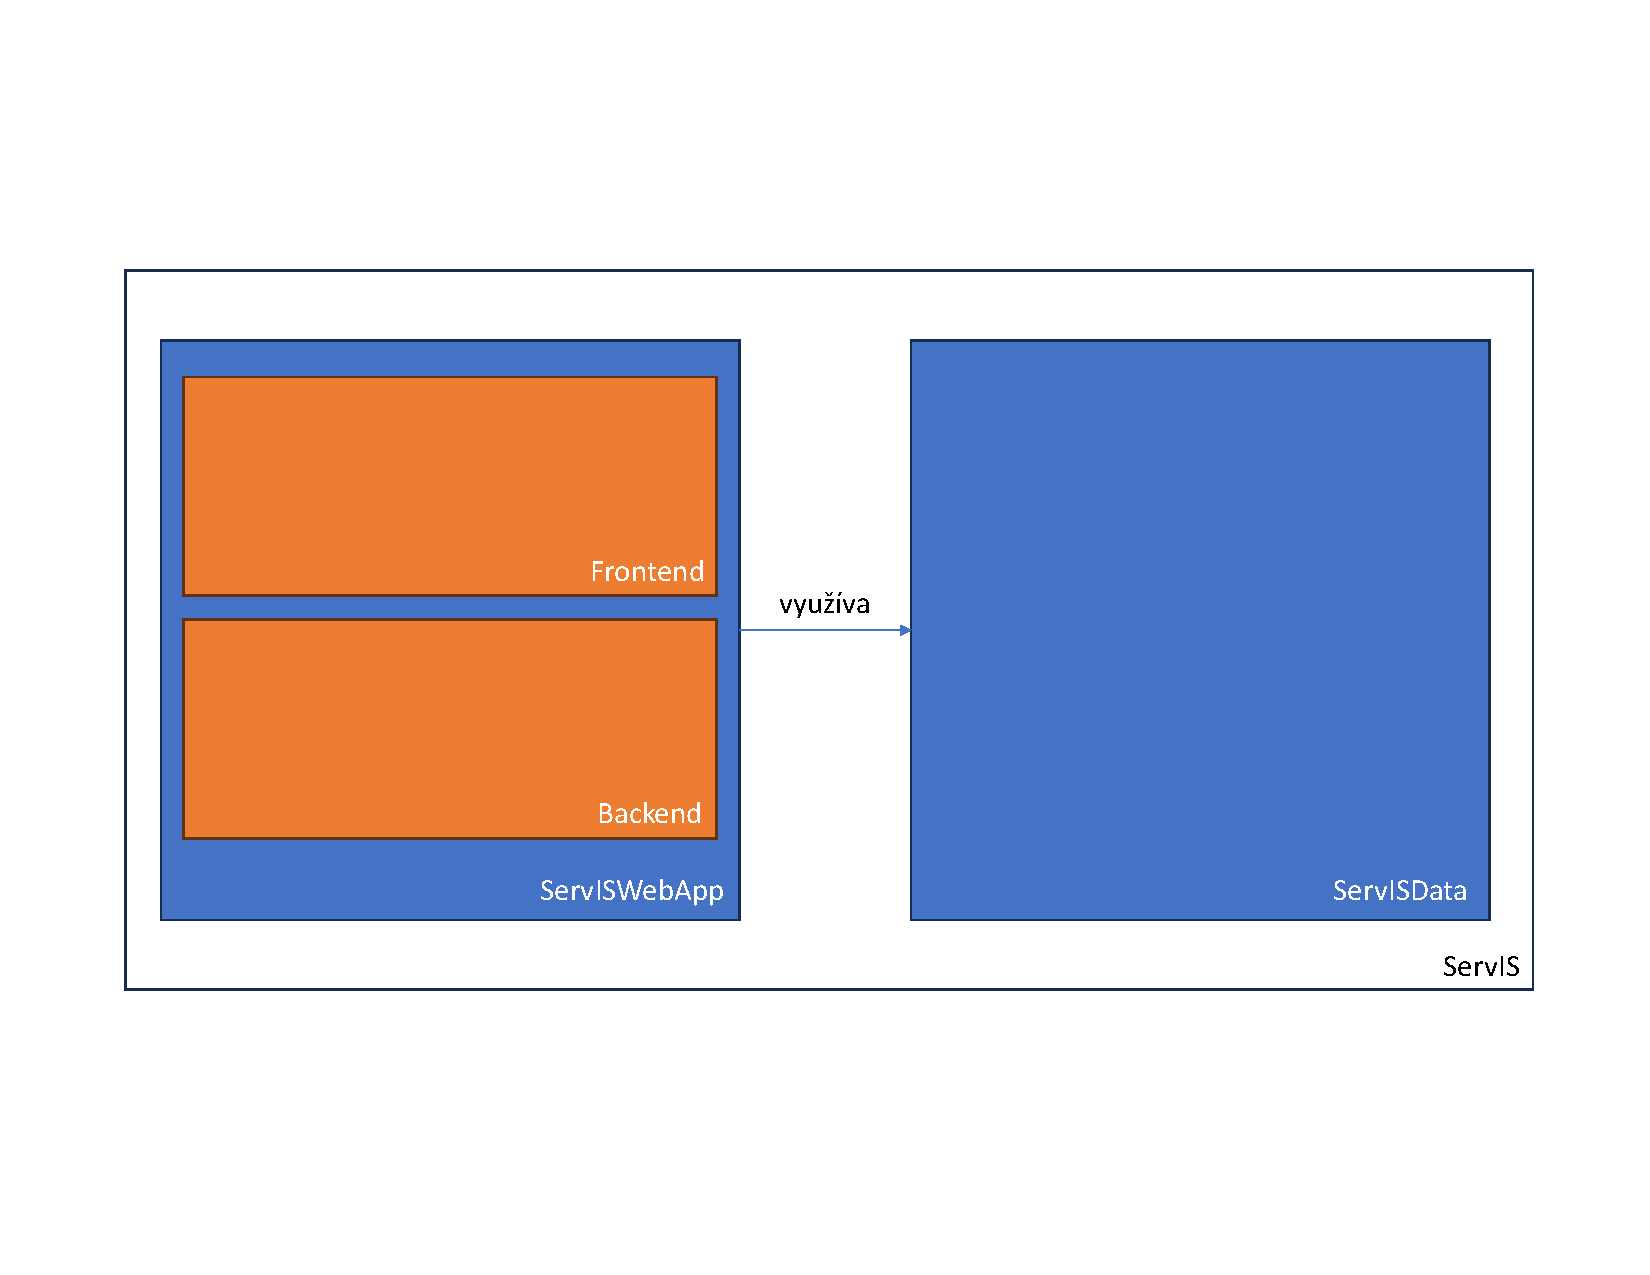
\includegraphics[width=140mm]{../img/architektura systemu}
\caption{Architektúra systému (predstavuje závislosť ServISWebApp od ServISData).}
\label{architektura systemu}
\end{figure}

\section{Voľba databázy}

Vieme, že náš systém potrebuje pre splnenie podmienok~P4, P5 a~P8 databázu. V tejto kapitole si vyberieme typ databázy, databazový server a~rozoberieme si aké entity potrebujeme.

\subsection{Návrh relačného modelu databázy}

Z P4 vieme, že potrebujeme entity pre bagre a~prídavné zariadenia. Niekoho by mohlo napadnúť spojiť obe entity do~jednej, ale to my nespravíme. Ide o~rozdielne entity, ktoré môžu uchovávať rozdielne informácie (a~ako neskôr v~texte uvidíme, skutočne budú uchovávať rozdielne dáta).

Kedže ide o~ponuku, ktorú chceme prezentovať zákazníkom, chceme okrem textových údajov prezentovať položku, či už stroj alebo~prídavné zariadenie, pomocou fotky. A~nie jednej (predpokladám, že položku budú chcieť firmy predviesť zákazníkom z viacerých uhlov). Znovu by niekomu mohlo napadnúť, že by bol dobrý nápad zlúčiť entitu fotky stroja s~entitou fotky prídavného zariadenia. Ale tieto veci nie sú totožné. Ak by sme entity zlúčili (a~mali teda iba 1 entitu pre~fotku všeobecne), tak by existovala možnosť priradiť fotku prídaného zariadenia stroju (a~naopak). Ale to je nesprávne. Preto znova vytvoríme dve entity. Jedna bude fotka stroja, druhá bude fotka prídavného zariadenia. Pre fotku stroja platí, že patrí práve jednému stroju. Stroj môže mať viacero fotiek. Analogicky platí pre prídavné zariadenia a~ich fotky.

Pri strojoch sa ešte zastavíme. Existujú rôzne značky strojov (napr. Locust, Eurocomach,\dots), a takisto rôzne ketegórie strojov (napr. šmykom riadené nakladače, pásové bagre,\dots). Ďalej v texte, keď budem používať spojenie typ stroja, tak tým myslím kombináciu značky stroja a kategórie stroja. Každý typ stroja sa môže líšiť druhom a formou údajov. Napríklad typ A má hmotnosť ako vlastnosť, ktorú chceme spolu so zbytkom údajov zobraziť užívateľovi. Ďalej typ B má namiesto hmotnosti údaj o výške stroja. Existujú údaje (ako sú napr. meno a opis stroja), ktoré existujú pre každý stroj. Ale takisto existujú údaje, ktoré sa líšia v závislosti od typu stroja. Takýmito údajmi sú vlastnosti stroja. Ako budeme tieto premenlivé údaje ukladať? Jedno z riešení, ktoré by nás mohlo napadnúť je vytvoriť rodičovskú entitu, ktorá by obsahovala údaje spoločné pre všetky typy strojov. A v entitách, ktoré by dedili od rodičovskej triedy by sme dodefinovali premenlivé vlastnosti. Toto riešenie by pravdepodobne fungovalo, lenže má zásadnú nevýhodu. Zakaždým keď si firma zmyslí, že potrebuje nový typ stroja, by entita musela byť manuálne doprogramovaná. Ale kedže my chceme systém navrhnúť všeobecne tak, aby si každá firma vedela zadefinovať vlastnú ponuku strojov, volíme inú alternatívu. Vytvoríme si entitu pre typ stroja. Každý stroj bude nejakého typu. Každý typ obsahuje údaj o~značke a~kategórii. Značka a~kategória sú tiež ďalšími entitami. Typ stroja určuje, akého typu budú vlastnosti konkrétneho stroja. Takže budeme potrebovať entitu typ vlastnosti stoja. Tá obsahuje údaje: názov vlastnosti (napr. hmotnosť, výška,\dots) a~typ hodnoty vlastnosti (napr. číslo, text,\dots). Teda admin bude môcť priradiť typu stroja akého typu bude mať konkrétny stroj vlastnosti.

Stroj vie svoj typ, a~ten vie aké (akého typu) má konkrétny stroj vlastnosti. To, čo ešte nevieme, sú konkrétne hodnoty vlastností stroja. Dovolím si vysvetliť na~príklade. Momentálne máme informáciu o~tom, že konkrétny stroj~S, typu~T, má vlasnosť hmotnosť, ale stále nevieme konkrétnu hodnotu, teda stále nevieme koľko váži. Preto vytvoríme entitu reprezentujúcu vlastnosť stroja. Táto entita vie, akého je typu. A~takisto v~sebe uchováva konkrétnu hodnotu vlastnosti (v~kontexte príkladu, uchováva v~sebe váhu stroja). Každý stroj má v~sebe toľko vlastností, koľko ich je zadefinovaných v~jeho type.

Teraz sa vráťme k~prídavným zariadeniam. Každé prídavné zariadenie má, podobne ako stroj, takisto svoju značku a~patrí do nejakej kategórie. Navyše má oproti strojom aj údaj o~tom, pre akú kategóriu strojov je zariadenie vytvorené. Avšak na rozdiel od~predošlého prípadu so~strojmi, sa tento prípad líši v~tom, že každé prídavné zariadenie, bez ohľadu na~kombináciu typu, kategórie a~kategórie stroja, má druh a~formu údajov rovnakú. Takže stačí ak vytvoríme entitu pre~značku a~kategóriu prídavného zariadenia (entitu pre kategóriu stroja už máme) a~entita reprezentujúca prídavné zariadenie si bude v~sebe držať informáciu o~tom, akej je značky, kategórie a~pre akú kategóriu strojov je vytvorená.

Aby sme splnili P5, budeme potrebovať entitu reprezentujúcu aukčnú ponuku. Aukčná ponuka bude držať informáciu o~tom, aký stroj je v~dražbe. A~takisto údaje o~ponuke (napr. vyvolávacia cena, koniec aukcie,\dots).

No okrem udržania údajov o~aukčnej ponuke a~draženom stroji, si musíme zapamätať i~údaje o~ponukách užívateľov, ktorý sa do~aukcie zapojili. Preto si vytvoríme entitu reprezentujúcu ponuku užívateľa. Bude v~sebe niesť údaje o~tom, ktorý úžívateľ ponúkol sumu, v~akej výške a~pre ktorú aukčnú ponuku.

Entitu užívateľa som načal už v~prechádzajúcom odstavci. Túto entitu skutočne budeme potrebovať a~to aj kvôli splneniu P8. Údaje užívateľov musíme pri~registrácii uchovať, aby sme nimi vedeli predvypĺniť formuláre, a~takisto aby sme vedeli vytvoriť prihlasovanie.

Čítateľ by mohol navrhnúť, že pre splnenie P6 budeme potrebovať entitu reprezentujúcu správy. Toto riešenie by mohlo fungovať, ale ako si neskôr ukážeme, existuje aj iné riešenie. Také, ktoré nám ušetrí úložisko v~databáze a navyše uľahčí implementáciu. Preto entitu pre správy nevytvárame.

Pre splnenie P7 si vytvoríme entitu, ktorá bude reprezentovať náhradné diely stroja. Každý náhradný diel bude niesť informáciu o~tom, v~ktorých strojoch sa nachádza. A~každý stroj bude vedieť aké diely obsahuje. Každý náhradný diel obsahuje katalógové číslo. Toto číslo je unikátne medzi strojmi, a~preto by mohlo byť použité ako primárny kľúč entity. Ale autor sa z opatrnosti a~kvôli konzistencii (každá entita má id) rozhodol využiť ako primárny kľúč id i~pri náhradných dieloch.

Hlavným predmetom predaja sú stroje. A~preto chceme aby prvé, čo zákazník po~príchode na~stránku uvidí bola ponuka strojov. Takže ešte budeme potrebovať entitu na~reprezentáciu hlavnej ponuky. Táto entita vie aký typ strojov ponúka, a~zároveň obsahuje reprezentatívnu fotku a~opis strojov daného typu.

Pre detailnejšiu predstavu môžeme návrh vidieť na~obrázku~\ref{relacny model uml}.

\begin{figure}[H]\centering
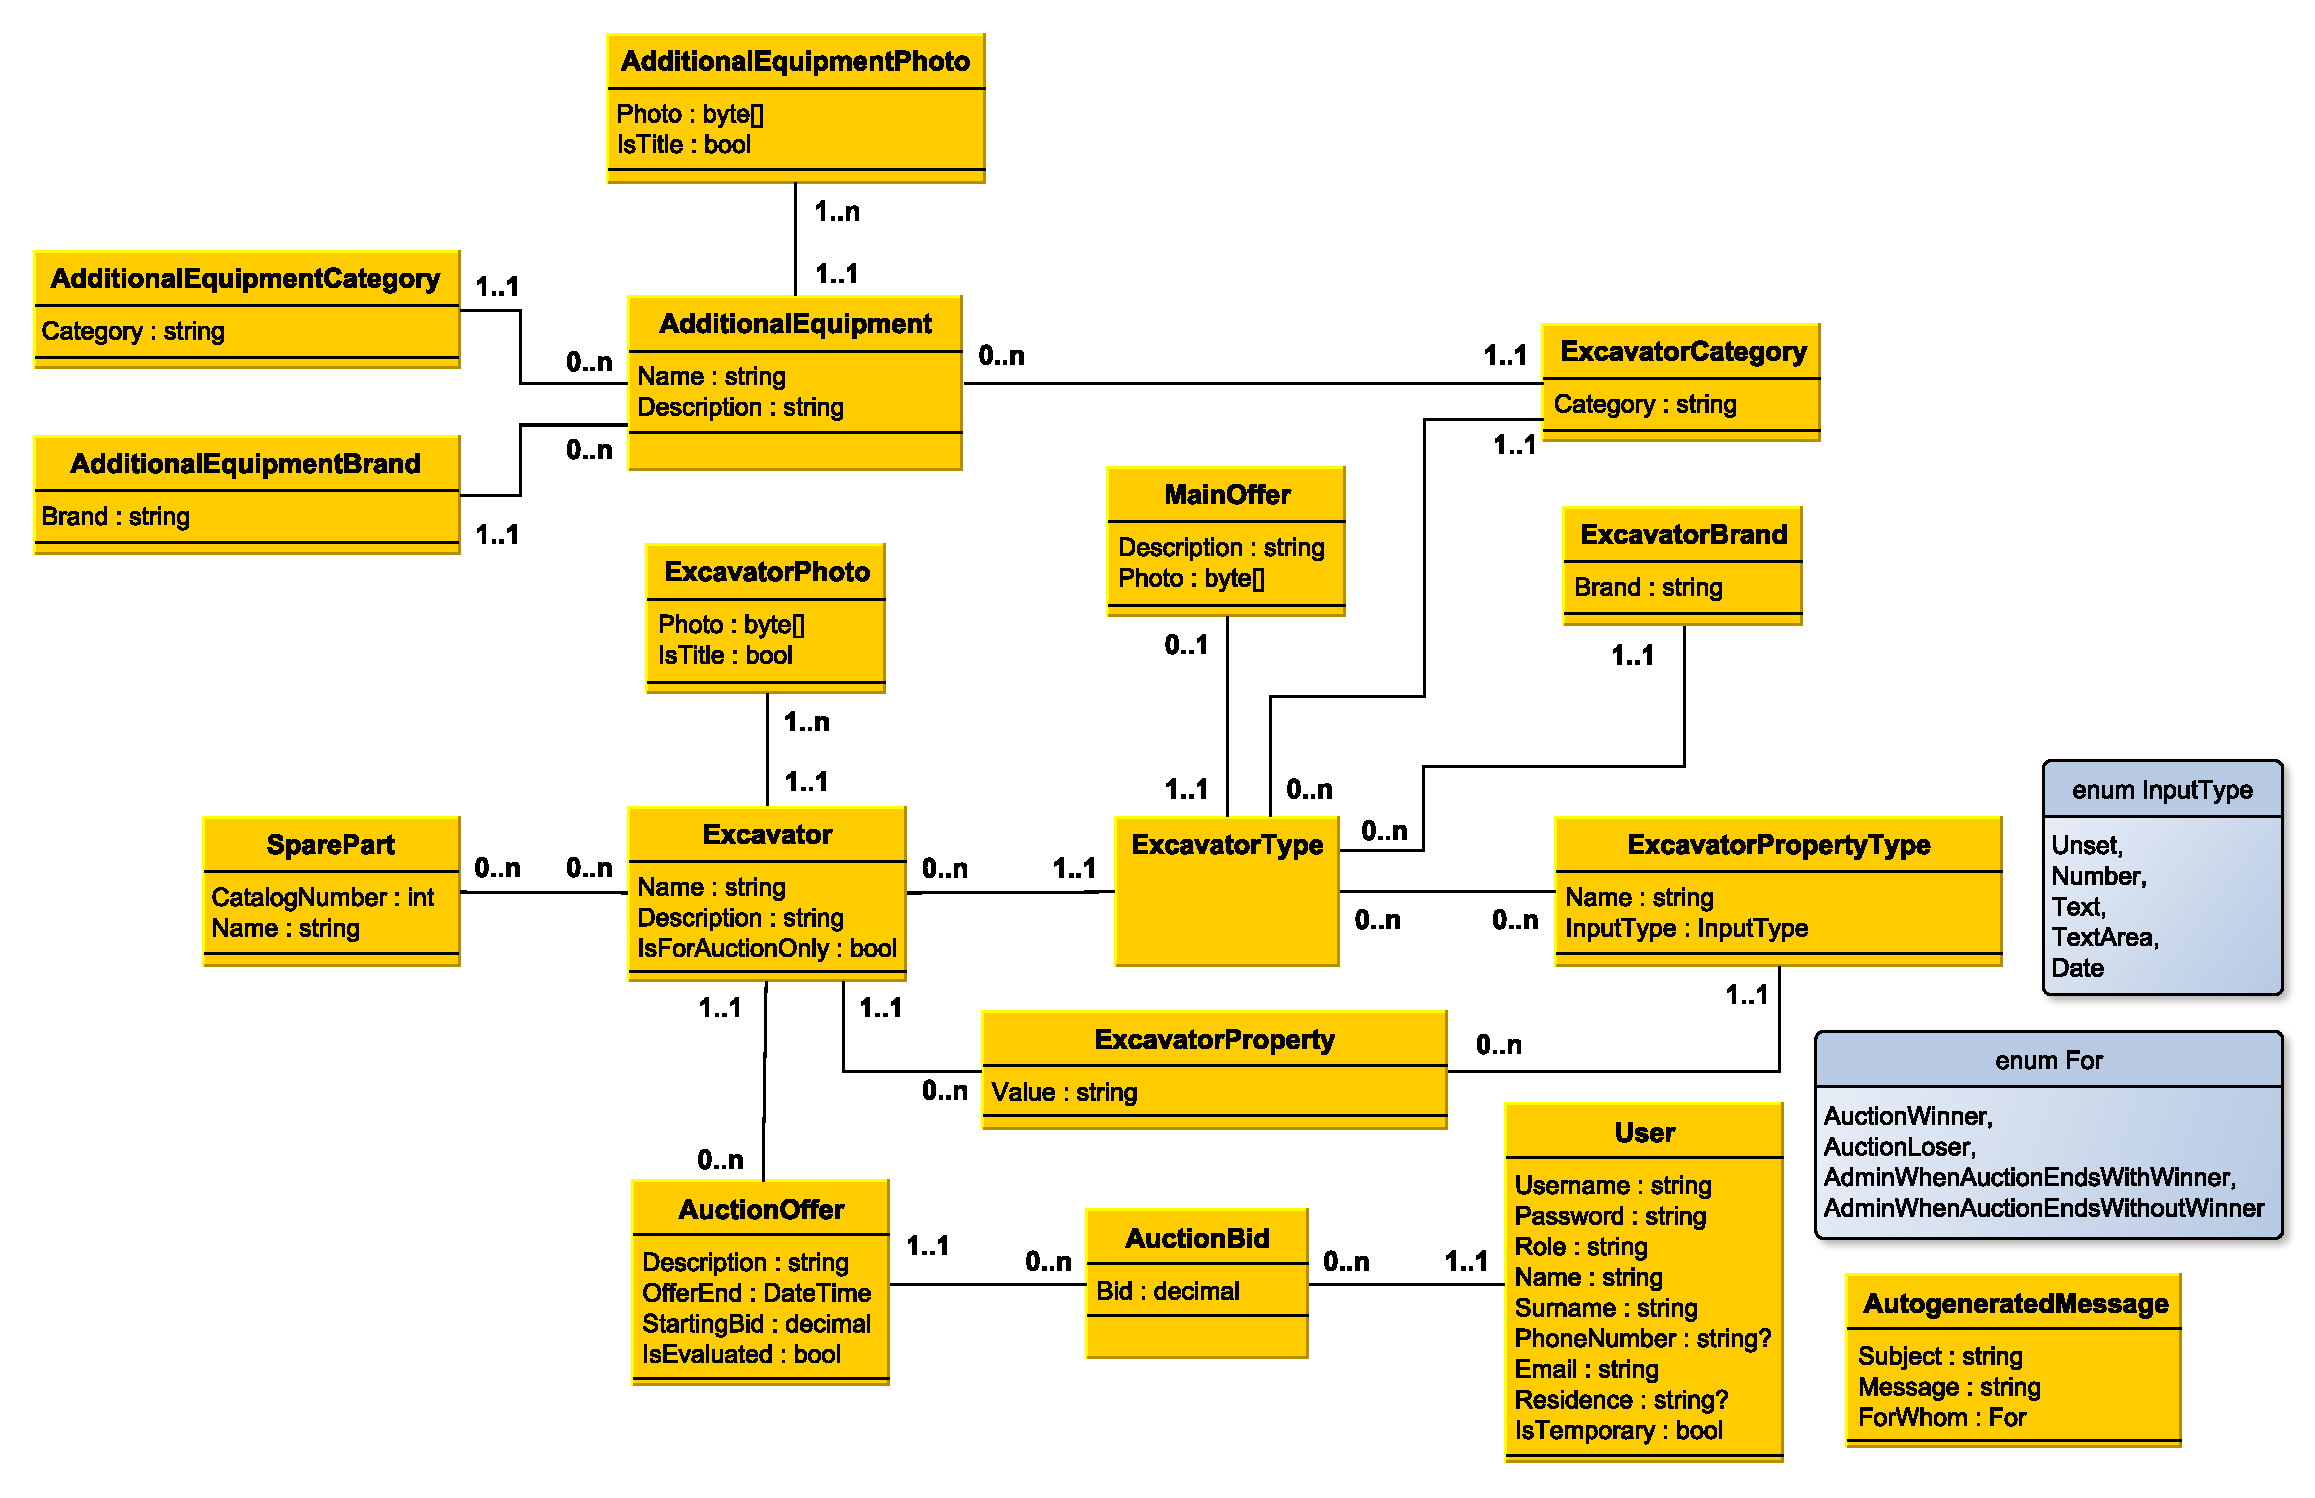
\includegraphics[width=140mm]{../img/relacny model uml}
\caption{Relačný model databázy.}
\label{relacny model uml}
\end{figure}

\subsection{Voľba typu databázy a databázového servera}

TBA

\subsection{ORM}

Prečo by sme chceli ORM.

\section{Aukcia- odpočet a vyhodnocovanie}

V tejto podkapitole predstavím BackgroundServices?, vysvetlím ako odpočítavať (len 1 timer, v osobitnej komponente kvôli rerenderom), ako funguje vyhodnocovanie- rozne scenare (co sa stane ak mame vitaza, co sa stane ak nemamee vitaza).

\section{Posielanie a príjimanie správ}

V tejto podkapitole rozoberieme spôsoby ako posielať/prijímať správy. Gmail api? AE.net? Mailkit?

% %%% Fiktivní kapitola s ukázkami sazby

\chapter{Nápověda k~sazbě}

\section{Úprava práce}

Vlastní text bakalářské práce je uspořádaný hierarchicky do kapitol a podkapitol,
každá kapitola začíná na nové straně. Text je zarovnán do bloku. Nový odstavec
se obvykle odděluje malou vertikální mezerou a odsazením prvního řádku. Grafická
úprava má být v~celém textu jednotná.

Práce se tiskne na bílý papír formátu A4. Okraje musí ponechat dost místa na vazbu:
doporučen je horní, dolní a pravý okraj $25\,\rm mm$, levý okraj $40\,\rm mm$.
Číslují se všechny strany kromě obálky a informačních stran na začátku práce;
první číslovaná strana bývá obvykle ta s~obsahem.

Písmo se doporučuje dvanáctibodové ($12\,\rm pt$) se standardní vzdáleností mezi řádky
(pokud píšete ve Wordu nebo podobném programu, odpovídá tomu řádkování $1,5$; v~\TeX{}u
není potřeba nic přepínat). Pro běžný text používejte vzpřímené patkové písmo.
Text matematických vět se obvykle tiskne pro zdůraznění skloněným (slanted) písmem,
není-li k~dispozici, může být zastoupeno kurzívou.

Primárně je doporučován jednostranný tisk (příliš tenkou práci lze obtížně svázat).
Delší práce je lepší tisknout oboustranně a přizpůsobit tomu velikosti okrajů:
$40\,\rm mm$ má vždy \emph{vnitřní} okraj. Rub titulního listu zůstává nepotištěný.

Zkratky použité v textu musí být vysvětleny vždy u prvního výskytu zkratky (v~závorce nebo
v poznámce pod čarou, jde-li o složitější vysvětlení pojmu či zkratky). Pokud je zkratek
více, připojuje se seznam použitých zkratek, včetně jejich vysvětlení a/nebo odkazů
na definici.

Delší převzatý text jiného autora je nutné vymezit uvozovkami nebo jinak vyznačit a řádně
citovat.

\section{Jednoduché příklady}

Čísla v~českém textu obvykle sázíme v~matematickém režimu s~desetinnou čárkou:
%%% Bez \usepackage{icomma}:
% $\pi \doteq 3{,}141\,592\,653\,589$.
%%% S \usepackage{icomma}:
$\pi \doteq 3,141\,592\,653\,589$.
V~matematických textech se považuje za přípustné používat desetinnou tečku
(pro lepší odlišení od čárky v~roli oddělovače). Numerické výsledky se uvádějí
s~přiměřeným počtem desetinných míst.

Mezi číslo a jednotku patří úzká mezera: šířka stránky A4 činí $210\,\rm mm$, což si
pamatuje pouze $5\,\%$ autorů. Pokud ale údaj slouží jako přívlastek, mezeru vynecháváme:
$25\rm mm$ okraj, $95\%$ interval spolehlivosti.

Rozlišujeme různé druhy pomlček:
červeno-černý (krátká pomlčka),
strana 16--22 (střední),
$45-44$ (matematické minus),
a~toto je --- jak se asi dalo čekat --- vložená věta ohraničená dlouhými pomlčkami.

V~českém textu se používají \uv{české} uvozovky, nikoliv ``anglické''.

% V tomto odstavci se vlnka zviditelňuje
{
\def~{{\tt\char126}}
Na některých místech je potřeba zabránit lámání řádku (v~\TeX{}u značíme vlnovkou):
u~předložek (neslabičnych, nebo obecně jednopísmenných), vrchol~$v$, před $k$~kroky,
a~proto, \dots{} obecně kdekoliv, kde by při rozlomení čtenář \uv{ško\-brt\-nul}.
}

\section{Matematické vzorce a výrazy}

Proměnné sázíme kurzívou (to \TeX{} v~matematickém módu dělá sám, ale
nezapomínejte na to v~okolním textu a také si matematický mód zapněte).
Názvy funkcí sázíme vzpřímeně. Tedy například:
$\var(X) = \E X^2 - \bigl(\E X \bigr)^2$.

Zlomky uvnitř odstavce (třeba $\frac{5}{7}$ nebo $\frac{x+y}{2}$) mohou
být příliš stísněné, takže je lepší sázet jednoduché zlomky s~lomítkem:
$5/7$, $(x+y)/2$.

Nechť
\[   % LaTeXová náhrada klasického TeXového $$
\mathbb{X} = \begin{pmatrix}
      \T{\bm x_1} \\
      \vdots \\
      \T{\bm x_n}
      \end{pmatrix}.
\]
Povšimněme si tečky za~maticí. Byť je matematický text vysázen
ve~specifickém prostředí, stále je gramaticky součástí věty a~tudíž je
zapotřebí neopomenout patřičná interpunkční znaménka. Výrazy, na které
chceme později odkazovat, je vhodné očíslovat:
\begin{equation}\label{eq01:Xmat}
\mathbb{X} = \begin{pmatrix}
      \T{\bm x_1} \\
      \vdots \\
      \T{\bm x_n}
      \end{pmatrix}.
\end{equation}
Výraz \eqref{eq01:Xmat} definuje matici $\mathbb{X}$. Pro lepší čitelnost
a~přehlednost textu je vhodné číslovat pouze ty výrazy, na které se
autor někde v~další části textu odkazuje. To jest, nečíslujte
automaticky všechny výrazy vysázené některým z~matematických
prostředí.

Zarovnání vzorců do několika sloupečků:
\begin{alignat*}{3}
S(t) &= \pr(T > t),    &\qquad t&>0       &\qquad&\text{ (zprava spojitá),}\\
F(t) &= \pr(T \leq t), &\qquad t&>0       &\qquad&\text{ (zprava spojitá).}
\end{alignat*}

Dva vzorce se spojovníkem:
\begin{equation}\label{eq01:FS}
\left.
\begin{aligned}
S(t) &= \pr(T > t) \\[1ex]
F(t) &= \pr(T \leq t)
\end{aligned}
\;	% zde pomůže ručně vynechat trochu místa
\right\}
\quad t>0 \qquad \text{(zprava spojité).}
\end{equation}

Dva centrované nečíslované vzorce:
\begin{gather*}
\bm Y = \mathbb{X}\bm\beta + \bm\varepsilon, \\[1ex]
\mathbb{X} = \begin{pmatrix} 1 & \T{\bm x_1} \\ \vdots & \vdots \\ 1 &
  \T{\bm x_n} \end{pmatrix}.
\end{gather*}
Dva centrované číslované vzorce:
\begin{gather}
\bm Y = \mathbb{X}\bm\beta + \bm\varepsilon, \label{eq02:Y}\\[1ex]
\mathbb{X} = \begin{pmatrix} 1 & \T{\bm x_1} \label{eq03:X}\\ \vdots & \vdots \\ 1 &
  \T{\bm x_n} \end{pmatrix}.
\end{gather}

Definice rozdělená na dva případy:
\[
P_{r-j}=
\begin{cases}
0, & \text{je-li $r-j$ liché},\\
r!\,(-1)^{(r-j)/2}, & \text{je-li $r-j$ sudé}.
\end{cases}
\]
Všimněte si použití interpunkce v této konstrukci. Čárky a tečky se
dávají na místa, kam podle jazykových pravidel patří.

\begin{align}
x& = y_1-y_2+y_3-y_5+y_8-\dots = && \text{z \eqref{eq02:Y}} \nonumber\\
& = y'\circ y^* = && \text{podle \eqref{eq03:X}} \nonumber\\
& = y(0) y' && \text {z Axiomu 1.}
\end{align}


Dva zarovnané vzorce nečíslované:
\begin{align*}
L(\bm\theta) &= \prod_{i=1}^n f_i(y_i;\,\bm\theta), \\
\ell(\bm\theta) &= \log\bigl\{L(\bm\theta)\bigr\} =
\sum_{i=1}^n \log\bigl\{f_i(y_i;\,\bm\theta)\bigr\}.
\end{align*}
Dva zarovnané vzorce, první číslovaný:
\begin{align}
L(\bm\theta) &= \prod_{i=1}^n f_i(y_i;\,\bm\theta), \label{eq01:L} \\
\ell(\bm\theta) &= \log\bigl\{L(\bm\theta)\bigr\} =
\sum_{i=1}^n \log\bigl\{f_i(y_i;\,\bm\theta)\bigr\}. \nonumber
\end{align}

Vzorec na dva řádky, první řádek zarovnaný vlevo, druhý vpravo, nečíslovaný:
\begin{multline*}
\ell(\mu,\,\sigma^2) = \log\bigl\{L(\mu,\,\sigma^2)\bigr\} =
\sum_{i=1}^n \log\bigl\{f_i(y_i;\,\mu,\,\sigma^2)\bigr\}= \\
  = -\,\frac{n}{2}\,\log(2\pi\sigma^2) \,-\,
\frac{1}{2\sigma^2}\sum_{i=1}^n\,(y_i - \mu)^2.
\end{multline*}

Vzorec na dva řádky, zarovnaný na $=$, číslovaný uprostřed:
\begin{equation}\label{eq01:ell}
\begin{split}
\ell(\mu,\,\sigma^2) &= \log\bigl\{L(\mu,\,\sigma^2)\bigr\} =
\sum_{i=1}^n \log\bigl\{f(y_i;\,\mu,\,\sigma^2)\bigr\}= \\
& = -\,\frac{n}{2}\,\log(2\pi\sigma^2) \,-\,
\frac{1}{2\sigma^2}\sum_{i=1}^n\,(y_i - \mu)^2.
\end{split}
\end{equation}

\section{Definice, věty, důkazy, \dots}

Konstrukce typu definice, věta, důkaz, příklad, \dots je vhodné
odlišit od okolního textu a~případně též číslovat s~možností použití
křížových odkazů. Pro každý typ těchto konstrukcí je vhodné mít
v~souboru s~makry (\texttt{makra.tex}) nadefinované jedno prostředí,
které zajistí jak vizuální odlišení od okolního textu, tak
automatické číslování s~možností křížově odkazovat.

\begin{definice}\label{def01:1}
  Nechť náhodné veličiny $X_1,\dots,X_n$ jsou definovány na témž
  prav\-dě\-po\-dob\-nost\-ním prostoru $(\Omega,\,\mathcal{A},\,\pr)$. Pak
  vektor $\bm X = \T{(X_1,\dots,X_n)}$ nazveme \emph{náhodným
    vektorem}.
\end{definice}

\begin{definice}[náhodný vektor]\label{def01:2}
  Nechť náhodné veličiny $X_1,\dots,X_n$ jsou definovány na témž
  pravděpodobnostním prostoru $(\Omega,\,\mathcal{A},\,\pr)$. Pak
  vektor $\bm X = \T{(X_1,\dots,X_n)}$ nazveme \emph{náhodným
    vektorem}.
\end{definice}
Definice~\ref{def01:1} ukazuje použití prostředí pro sazbu definice
bez titulku, definice~\ref{def01:2} ukazuje použití prostředí pro
sazbu definice s~titulkem.

\begin{veta}\label{veta01:1}
  Náhodný vektor $\bm X$ je měřitelné zobrazení prostoru
  $(\Omega,\,\mathcal{A},\,\pr)$ do $(\R_n,\,\mathcal{B}_n)$.
\end{veta}

\begin{lemma}[\citealp{Andel07}, str. 29]\label{veta01:2}
  Náhodný vektor $\bm X$ je měřitelné zobrazení prostoru
  $(\Omega,\,\mathcal{A},\,\pr)$ do $(\R_n,\,\mathcal{B}_n)$.
\end{lemma}
\begin{dukaz}
  Jednotlivé kroky důkazu jsou podrobně popsány v~práci \citet[str.
  29]{Andel07}.
\end{dukaz}
Věta~\ref{veta01:1} ukazuje použití prostředí pro sazbu matematické
věty bez titulku, lemma~\ref{veta01:2} ukazuje použití prostředí pro
sazbu matematické věty s~titulkem. Lemmata byla zavedena v~hlavním
souboru tak, že sdílejí číslování s~větami.

% %%% Fiktivní kapitola s ukázkami citací

\chapter{Odkazy na literaturu}

Odkazy na literaturu vytváříme nejlépe pomocí příkazů
\verb|\citet|, \verb|\citep| atp.
(viz {\LaTeX}ový balíček \textsf{natbib}) a~následného použití
Bib{\TeX}u. V~matematickém textu obvykle odkazujeme stylem \uv{Jméno
autora/autorů (rok vydání)}, resp. \uv{Jméno autora/autorů [číslo
odkazu]}. V~českém/slovenském textu je potřeba se navíc vypořádat
s~nutností skloňovat jméno autora, respektive přechylovat jméno
autorky. Je potřeba mít na paměti, že standardní příkazy
\verb|\citet|, \verb|\citep|
produkují referenci se jménem autora/autorů v~prvním pádě a~jména
autorek jsou nepřechýlena.

Pokud nepoužíváme bib\TeX{}, řídíme se normou ISO 690 a zvyklostmi
oboru.

Jména časopisů lze uvádět zkráceně, ale pouze v~kodifikované podobě.

\section{Několik ukázek}

Mezi nejvíce citované statistické články patří práce Kaplana a~Meiera a~Coxe
\citep{KaplanMeier58, Cox72}. \citet{Student08} napsal článek o~t-testu.

Prof. Anděl je autorem učebnice matematické statistiky
\citep[viz][]{Andel98}. Teorii odhadu se věnuje práce
\citet{LehmannCasella98}. V~případě odkazů na specifickou informaci
(definice, důkaz, \dots) uvedenou v~knize bývá užitečné uvést
specificky číslo kapitoly, číslo věty atp. obsahující požadovanou
informaci, např. viz \citet[Věta 4.22]{Andel07} nebo \citep[viz][Věta
4.22]{Andel07}.

Mnoho článků je výsledkem spolupráce celé řady osob. Při odkazování
v~textu na článek se třemi autory obvykle při prvním výskytu uvedeme
plný seznam: \citet*{DempsterLairdRubin77} představili koncept EM
algoritmu. Respektive: Koncept EM algoritmu byl představen v~práci
Dempstera, Lairdové a~Rubina \citep*{DempsterLairdRubin77}. Při každém
dalším výskytu již používáme zkrácenou verzi:
\citet{DempsterLairdRubin77} nabízejí též několik příkladů použití EM
algoritmu. Respektive: Několik příkladů použití EM algoritmu lze
nalézt též v~práci Dempstera a~kol. \citep{DempsterLairdRubin77}.

U~článku s~více než třemi autory odkazujeme vždy zkrácenou formou:
První výsledky projektu ACCEPT jsou uvedeny v~práci Genbergové a~kol.
\citep{Genberget08}. V~textu \emph{nenapíšeme}: První výsledky
projektu ACCEPT jsou uvedeny v~práci \citet*{Genberget08}.

% %%% Fiktivní kapitola s ukázkami tabulek, obrázků a kódu

\chapter{Tabulky, obrázky, programy}

Používání tabulek a grafů v~odborném textu má některá společná
pravidla a~některá specifická. Tabulky a grafy neuvádíme přímo do
textu, ale umístíme je buď na samostatné stránky nebo na vyhrazené
místo v~horní nebo dolní části běžných stránek. \LaTeX\ se o~umístění
plovoucích grafů a tabulek postará automaticky.

Každý graf a tabulku
očíslujeme a umístíme pod ně legendu. Legenda má popisovat obsah grafu
či tabulky tak podrobně, aby jim čtenář rozuměl bez důkladného
studování textu práce.

Na každou tabulku a graf musí být v~textu odkaz
pomocí jejich čísla. Na příslušném místě textu pak shrneme ty
nejdůležitější závěry, které lze z~tabulky či grafu učinit. Text by
měl být čitelný a srozumitelný i~bez prohlížení tabulek a grafů a
tabulky a grafy by měly být srozumitelné i~bez podrobné četby textu.

Na tabulky a grafy odkazujeme pokud možno nepřímo v~průběhu běžného
toku textu; místo \emph{\uv{Tabulka~\ref{tab03:Nejaka} ukazuje, že
    muži jsou v~průměru o~$9,9\,\rm kg$ těžší než ženy}} raději napíšeme
\emph{\uv{Muži jsou o~$9,9\,\rm kg$ těžší než ženy (viz
    Tabulka~\ref{tab03:Nejaka})}}.

\section{Tabulky}

\begin{table}[b!]

\centering
%%% Tabulka používá následující balíčky:
%%%   - booktabs (\toprule, \midrule, \bottomrule)
%%%   - dcolumn (typ sloupce D: vycentrovaná čísla zarovnaná na
%%%     desetinnou čárku
%%%     Všimněte si, že ve zdrojovém kódu jsou desetinné tečky, ale
%%%     tisknou se čárky.
%%% Dále používáme příkazy \pulrad a \mc definované v makra.tex

\begin{tabular}{l@{\hspace{1.5cm}}D{.}{,}{3.2}D{.}{,}{1.2}D{.}{,}{2.3}}
\toprule
 & \mc{} & \mc{\textbf{Směrod.}} & \mc{} \\
\pulrad{\textbf{Efekt}} & \mc{\pulrad{\textbf{Odhad}}} & \mc{\textbf{chyba}$^a$} &
\mc{\pulrad{\textbf{P-hodnota}}} \\
\midrule
Abs. člen     & -10.01 & 1.01 & \mc{---} \\
Pohlaví (muž) & 9.89   & 5.98 & 0.098 \\
Výška (cm)    & 0.78   & 0.12 & <0.001 \\
\bottomrule
\multicolumn{4}{l}{\footnotesize \textit{Pozn:}
$^a$ Směrodatná chyba odhadu metodou Monte Carlo.}
\end{tabular}

\caption{Maximálně věrohodné odhady v~modelu M.}\label{tab03:Nejaka}

\end{table}

U~\textbf{tabulek} se doporučuje dodržovat následující pravidla:

\begin{itemize} %% nebo compactitem z balíku paralist
\item Vyhýbat se svislým linkám. Silnějšími vodorovnými linkami
  oddělit tabulku od okolního textu včetně legendy, slabšími
  vodorovnými linkami oddělovat záhlaví sloupců od těla tabulky a
  jednotlivé části tabulky mezi sebou. V~\LaTeX u tuto podobu tabulek
  implementuje balík \texttt{booktabs}. Chceme-li výrazněji oddělit
  některé sloupce od jiných, vložíme mezi ně větší mezeru.
\item Neměnit typ, formát a význam obsahu políček v~tomtéž sloupci
  (není dobré do téhož sloupce zapisovat tu průměr, onde procenta).
\item Neopakovat tentýž obsah políček mnohokrát za sebou. Máme-li
  sloupec \textit{Rozptyl}, který v~prvních deseti řádcích obsahuje
  hodnotu $0,5$ a v~druhých deseti řádcích hodnotu $1,5$, pak tento
  sloupec raději zrušíme a vyřešíme to jinak. Například můžeme tabulku
  rozdělit na dvě nebo do ní vložit popisné řádky, které informují
o~nějaké proměnné hodnotě opakující se v~následujícím oddíle tabulky
  (např. \emph{\uv{Rozptyl${}=0,5$}} a níže \emph{\uv{Rozptyl${}=
      1,5$}}).
\item Čísla v~tabulce zarovnávat na desetinnou čárku.
\item V~tabulce je někdy potřebné používat zkratky, které se jinde
nevyskytují. Tyto zkratky můžeme vysvětlit v~legendě nebo
v~poznámkách pod tabulkou. Poznámky pod tabulkou můžeme využít i
k~podrobnějšímu vysvětlení významu  některých sloupců nebo hodnot.
\end{itemize}

\section{Obrázky}

Několik rad týkajících se obrázků a grafů.

\begin{itemize}
\item Graf by měl být vytvořen ve velikosti, v~níž bude použit
  v~práci. Zmenšení příliš velkého grafu vede ke špatné čitelnosti
  popisků.
\item Osy grafu musí být řádně popsány ve stejném jazyce, v~jakém je
  psána práce (absenci diakritiky lze tolerovat). Kreslíme-li graf
  hmotnosti proti výšce, nenecháme na nich popisky \texttt{ht} a
  \texttt{wt}, ale osy popíšeme \emph{Výška [cm]} a~\emph{Hmotnost
    [kg]}. Kreslíme-li graf funkce $h(x)$, popíšeme osy $x$ a $h(x)$.
  Každá osa musí mít jasně určenou škálu.
\item Chceme-li na dvourozměrném grafu vyznačit velké množství bodů,
  dáme pozor, aby se neslily do jednolité černé tmy. Je-li bodů mnoho,
  zmenšíme velikost symbolu, kterým je vykreslujeme, anebo vybereme
  jen malou část bodů, kterou do grafu zaneseme. Grafy, které obsahují
  tisíce bodů, dělají problémy hlavně v~elektronických dokumentech,
  protože výrazně zvětšují velikost souborů.
\item Budeme-li práci tisknout černobíle, vyhneme se používání barev.
  Čáry roz\-li\-šu\-je\-me typem (plná, tečkovaná, čerchovaná,\ldots), plochy
  dostatečně roz\-díl\-ný\-mi intensitami šedé nebo šrafováním. Význam
  jednotlivých typů čar a~ploch vysvětlíme buď v~textové legendě ke
  grafu anebo v~grafické legendě, která je přímo součástí obrázku.
\item Vyhýbejte se bitmapovým obrázkům o~nízkém rozlišení a zejména
  JPEGům (zuby a kompresní artefakty nevypadají na papíře pěkně).
  Lepší je vytvářet obrázky vektorově a vložit do textu jako PDF.
\end{itemize}

\section{Programy}

Algoritmy, výpisy programů a popis interakce s~programy je vhodné
odlišit od ostatního textu. Jednou z~možností je použití {\LaTeX}o\-vé\-ho balíčku
\texttt{fancyvrb} (fancy verbatim), pomocí něhož je v~souboru \texttt{makra.tex}
nadefinováno prostředí \texttt{code}. Pomocí něho lze vytvořit
např. následující ukázky.

\begin{code}
> mean(x)
[1] 158.90
> objekt$prumer
[1] 158.90
\end{code}
%$
Menší písmo:
\begin{code}[fontsize=\footnotesize]
> mean(x)
[1] 158.90
> objekt$prumer
[1] 158.90
\end{code}
%$
Bez rámečku:
\begin{code}[frame=none]
> mean(x)
[1] 158.90
> objekt$prumer
[1] 158.90
\end{code}
%$
Užší rámeček:
\begin{code}[xrightmargin=20em]
> mean(x)
[1] 158.90
> objekt$prumer
[1] 158.90
\end{code}
%$

\begin{figure}[p]\centering
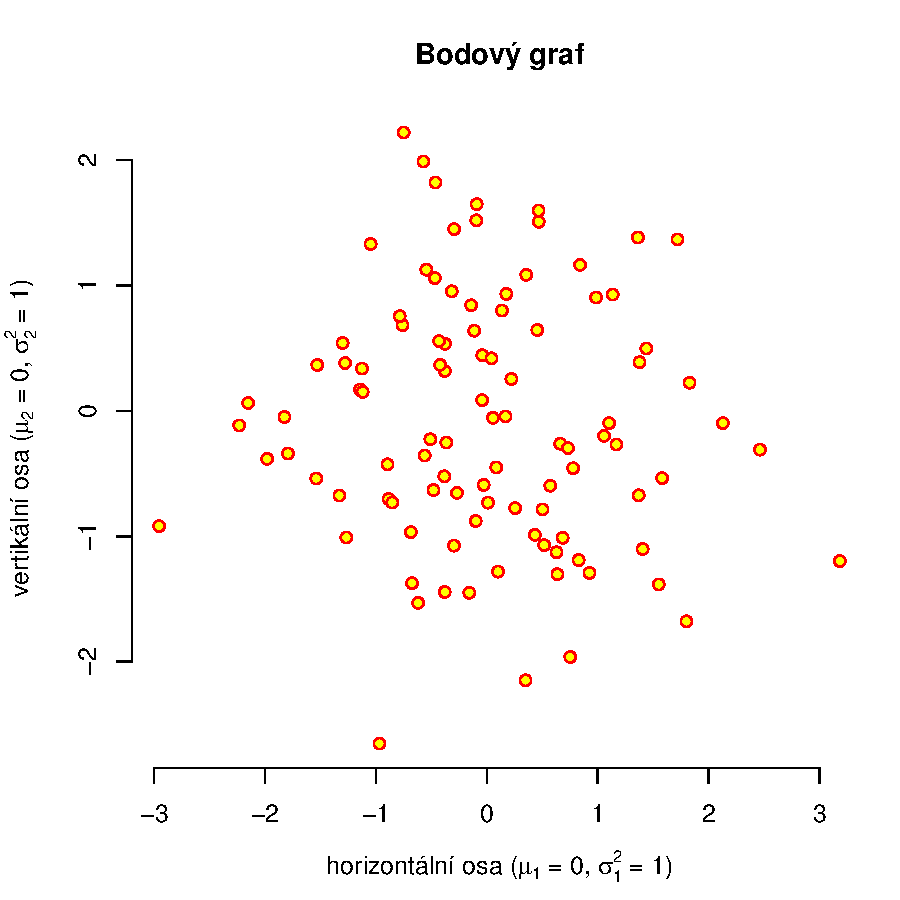
\includegraphics[width=140mm, height=140mm]{../img/ukazka-obr01}
% Příponu není potřeba explicitně uvádět, pdflatex automaticky hledá pdf.
% Rozměry také není nutné uvádět.
\caption{Náhodný výběr z~rozdělení $\mathcal{N}_2(\boldsymbol{0},\,I)$.}
\label{obr03:Nvyber}

\end{figure}

\begin{figure}[p]\centering
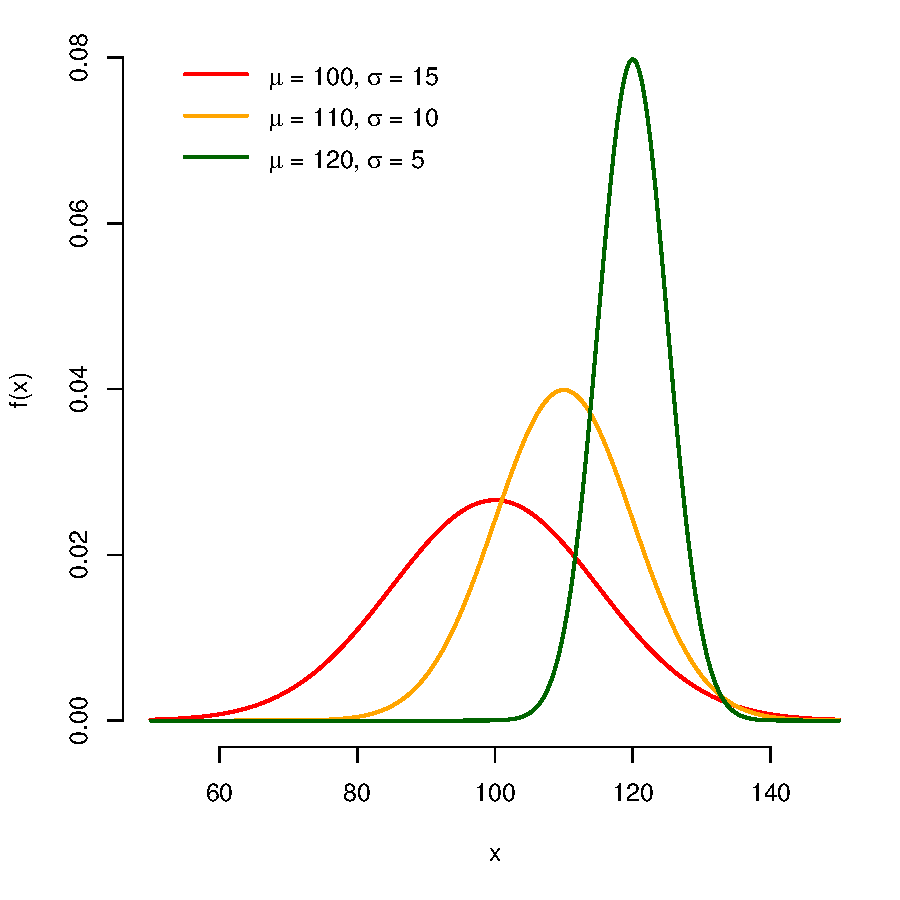
\includegraphics[width=140mm, height=140mm]{../img/ukazka-obr02}
\caption{Hustoty několika normálních rozdělení.}
\label{obr03:Nhust}
\end{figure}

\begin{figure}[p]\centering
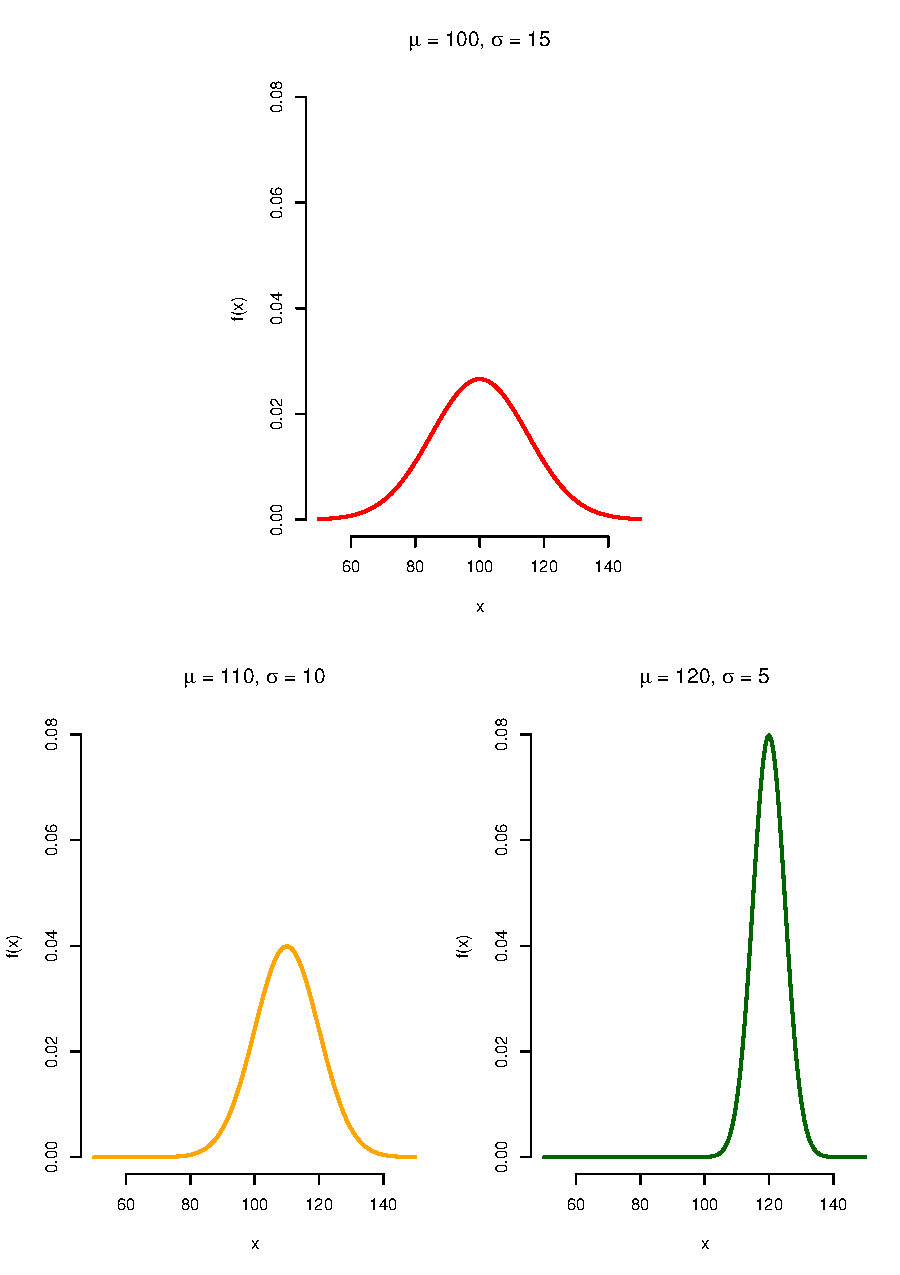
\includegraphics[width=140mm, height=198mm]{../img/ukazka-obr03}
\caption{Hustoty několika normálních rozdělení.}
\label{obr03:Nhust:podruhe}

\end{figure}

% %%% Fiktivní kapitola s instrukcemi k PDF/A

\chapter{Formát PDF/A}

Opatření rektora č. 13/2017 určuje, že elektronická podoba závěrečných
prací musí být odevzdávána ve formátu PDF/A úrovně 1a nebo 2u. To jsou
profily formátu PDF určující, jaké vlastnosti PDF je povoleno používat,
aby byly dokumenty vhodné k~dlouhodobé archivaci a dalšímu automatickému
zpracování. Dále se budeme zabývat úrovní 2u, kterou sázíme \TeX{}em.

Mezi nejdůležitější požadavky PDF/A-2u patří:

\begin{itemize}

\item Všechny fonty musí být zabudovány uvnitř dokumentu. Nejsou přípustné
odkazy na externí fonty (ani na \uv{systémové}, jako je Helvetica nebo Times).

\item Fonty musí obsahovat tabulku ToUnicode, která definuje převod z~kódování
znaků použitého uvnitř fontu to Unicode. Díky tomu je možné z~dokumentu
spolehlivě extrahovat text.

\item Dokument musí obsahovat metadata ve formátu XMP a je-li barevný,
pak také formální specifikaci barevného prostoru.

\end{itemize}

Tato šablona používá balíček {\tt pdfx,} který umí \LaTeX{} nastavit tak,
aby požadavky PDF/A splňoval. Metadata v~XMP se generují automaticky podle
informací v~souboru {\tt prace.xmpdata} (na vygenerovaný soubor se můžete
podívat v~{\tt pdfa.xmpi}).

Validitu PDF/A můžete zkontrolovat pomocí nástroje VeraPDF, který je
k~dispozici na \url{http://verapdf.org/}.

Pokud soubor nebude validní, mezi obvyklé příčiny patří používání méně
obvyklých fontů (které se vkládají pouze v~bitmapové podobě a/nebo bez
unicodových tabulek) a vkládání obrázků v~PDF, které samy o~sobě standard
PDF/A nesplňují.

Další postřehy o~práci s~PDF/A najdete na \url{http://mj.ucw.cz/vyuka/bc/pdfaq.html}.


\chapter*{Záver}
\addcontentsline{toc}{chapter}{Záver}

V~závere zhodnotíme ako sa nám podarilo naplniť požiadavky definované v~Úvode, konkrétne v~podkapitole~Požiadavky na~softvér~(\ref{poziadavky}).

\begin{itemize}
\item \textbf{P1 Dostupnosť}

Náš systém je webovou aplikáciou, ktorá je dostupná pre~užívateľov odkiaľkoľvek (samozrejme za~predpokladu, že majú prístup k~internetu).

\item \textbf{P2 Náklady}

Všetky balíčky využívané aplikáciou sú buď úplne zdarma alebo~využívame ich bezplatné verzie. Čo sa týka databázového servera, tak ten takisto využívame v~jeho bezplatnej verzii.

\item \textbf{P3 Minimálna obsluha softvéru}

Táto požiadavka sa odzrkadľuje v~správaní aukcie. V~prípade, že aukčná ponuka skončí bez~toho, aby sa jej niekto účastnil, posunie sa jej termín ukončenia aj bez~zásahu administrátora.

\item \textbf{P4 Predstavenie ponuky zákazníkom}

Systém je schopný načítať z~databázy dáta strojov aj prídavných zariadení a~zobraziť ich užívateľom.

\item \textbf{P5 Aukcia}

V~aplikácií existuje aukcia strojov. Administrátorom je umožnené vytvárať aukčne ponuky, v~ktorých sa draží (adminom vybraný) stroj. Užívateľom je v~prípade záujmu umožnené ponúkať sumy do~dražby. Po~skončení odpočtu prebehne vyhodnocovanie aukčných ponúk, kde sa rozhodne kto je ich víťazom. Víťaz je oboznámený prostredníctvom emailu, že vyhral. Porazení sú informovaní o~skutočnosti, že sa im aukciu nepodarilo vyhrať. Admin je upozornený, že aukčná ponuka skončila a~kto je jej víťazom.

\item \textbf{P6 Dopyt}

Systém umožňuje užívateľom podávať dopyt prostredníctvom formulára, ktorý odošle email administrátorovi s~potrebnými informáciami o~užívateľovi a~jeho záujme o~danú položku.

\item \textbf{P7 Prístup k súčiastkam strojov}

V~aplikácií si vie administrátor po~kliknutí na~profil v~správe strojov rozkliknúť detail nejakého konkrétneho stroja. Okrem iných údajov o~spomínanom stroji sa mu zobrazí aj zoznam náhradných dielov, ktoré stroj obsahuje.

\item \textbf{P8 Registrácia a prihlásenie užívateľov}

Systém umožňuje bežným užívateľom vytvoriť si účet v~systéme, a~takisto sa doň prihlásiť (možnosť odhlásenia je samozrejmosťou). A~po~prihlásení už nemusia do~formulárov (pri posielaní dopytu alebo pri~zapájani sa do~aukcie) zadávať svoje údaje.
\end{itemize}

\section{GDPR}

Keďže je náš systém webovou aplikáciou zhromažďujúcou užívateľské údaje, tak je potrebné riešiť zásady ochrany osobných údajov. Autor nie je právnikom, a~teda nemôže oficiálne prehlásiť, že systém je v~súlade s~GDPR\footnote{\url{https://en.wikipedia.org/wiki/General_Data_Protection_Regulation}}. Ale systém bol navrhnutý tak, aby zásady splnil. Užívateľa upozorňuje na~podmienky a~zásady používania systému. Takisto užívateľovi umožnuje vlastné dáta zmazať zo~systému, zobraziť a~exportovať ich na~vyžiadanie. Dáta síce nie sú šifrované softvérovo, ale táto podmienka sa dá splniť pri~výbere hostingu. Stačí si vybrať hosting, ktorý ponúka disky podporujúce šifrovanie dát.

\section{Možné vylepšenia}

Softvér síce spĺňa požiadavky a~jeho funkčnosť je dostatočná, ale stále existuje priestor pre~rôzne vylepšenia a~pridanie nových funkcionalít. V~tejto podkapitole si o~niektorých povieme.

\begin{itemize}
\item \textbf{Výkonnosť listovania ponuky}

Ponuku firmy (napr.~stroje) prečítame z~databázy a~vylistujeme jednotlívé položky. Nevyužívame žiadnu virtualizáciu, ani~stránkovanie. Keďže systém je určený pre~malé firmy a~nepredpokladá sa veľká ponuka, tak táto skutočnosť nepredstavuje problem. No v~budúcnosti, ak by sa firme používajúcej náš systém darilo a~rozhodla by sa rozšíriť ponuku, mohla by sa virtualizácia alebo~stránkovanie hodiť.

\item \textbf{Vylepšenie manažovania správ}

Systém síce umožňuje administrátorovi~prijímať emaily, a~takisto na~nich odpovedať, mazať ich, a~tiež označovať správy ako prečítané/neprečítané. No je v~tom trocha pomalý. Akcie síce netrvajú hodiny, a~ani minúty, ale do budúcna je to určite niečo, na~čom by bolo dobré popracovať.

Takisto by bolo dobré správam pridať~stránkovanie, vyhľadávanie a~triedenie podľa dátumu. Hlavným dôvodom existencie správ je umožniť administrátorovi reagovať na~dopyt užívateľov, a~takisto admina upozorňovať na~stav aukčných ponúk. Z~podstaty obsahu správ sa čas na~ich vybavenie odhaduje na~jednotky dní. A~teda predpokladáme, že počet správ v~schránke nebude príliš vysoký. V~prípade, že by ich admin nemazal stále platí, že relevantné správy sa budú nachádzať na~vrchu schránky. Ako vidíme, spomínané vlastnosti preto nie sú pre~naše účely nevyhnutné. Ale takisto ide o~funkcionality, ktoré by mohli oceniť firmy obzvlášť v~budúcnosti, kedy by sa zvýšením počtu zákazníkov zvýšila aj~frakvencia prichádzajúcich správ.

\item \textbf{Upozornenie na prehliadku stroja}

Vo~svete to funguje tak, že keď si užívateľ zakúpi stroj, tak po~určitom čase by firma mala prísť na~prehliadku a~stroj skontrolovať. Preto by sme do~nášho systému mohli pridať funkcionalitu, ktorá by fungovala následovne. Ak užívateľ odošle dopyt na~nejaký stroj a~obchod prebehne úspešne, admin by túto skutočnosť zaznačil v~systéme, čím by užívateľovi priradil dopytovaný stroj. Potom by sa spustil časovač, ktorý by po~uplynutí definovaného času upozornil administrátora na~blížiacu sa prehliadku.
\end{itemize}


%%% Seznam použité literatury
%%% Seznam použité literatury (bibliografie)
%%%
%%% Pro vytváření bibliografie používáme bibTeX. Ten zpracovává
%%% citace v textu (např. makro \cite{...}) a vyhledává k nim literaturu
%%% v souboru literatura.bib.
%%%
%%% Příkaz \bibliographystyle určuje, jakým stylem budou citovány odkazy
%%% v textu. V závorce je název zvoleného souboru .bst. Styly plainnat
%%% a unsrt jsou standardní součástí latexových distribucí. Styl czplainnat
%%% je dodáván s touto šablonou a bibTeX ho hledá v aktuálním adresáři.

\bibliographystyle{czplainnat}    %% Autor (rok) s českými spojkami
% \bibliographystyle{plainnat}    %% Autor (rok) s anglickými spojkami
% \bibliographystyle{unsrt}       %% [číslo]

\renewcommand{\bibname}{Seznam použité literatury}

%%% Vytvoření seznamu literatury. Pozor, pokud jste necitovali ani jednu
%%% položku, seznam se automaticky vynechá.

\bibliography{literatura}

%%% Kdybyste chtěli bibliografii vytvářet ručně (bez bibTeXu), lze to udělat
%%% následovně. V takovém případě se řiďte normou ISO 690 a zvyklostmi v oboru.

% \begin{thebibliography}{99}
%
% \bibitem{lamport94}
%   {\sc Lamport,} Leslie.
%   \emph{\LaTeX: A Document Preparation System}.
%   2. vydání.
%   Massachusetts: Addison Wesley, 1994.
%   ISBN 0-201-52983-1.
%
% \end{thebibliography}


%%% Obrázky v bakalářské práci
%%% (pokud jich je malé množství, obvykle není třeba seznam uvádět)
% \listoffigures

%%% Tabulky v bakalářské práci (opět nemusí být nutné uvádět)
%%% U matematických prací může být lepší přemístit seznam tabulek na začátek práce.
% \listoftables

%%% Použité zkratky v bakalářské práci (opět nemusí být nutné uvádět)
%%% U matematických prací může být lepší přemístit seznam zkratek na začátek práce.
% \chapwithtoc{Seznam použitých zkratek}

%%% Přílohy k bakalářské práci, existují-li. Každá příloha musí být alespoň jednou
%%% odkazována z vlastního textu práce. Přílohy se číslují.
%%%
%%% Do tištěné verze se spíše hodí přílohy, které lze číst a prohlížet (dodatečné
%%% tabulky a grafy, různé textové doplňky, ukázky výstupů z počítačových programů,
%%% apod.). Do elektronické verze se hodí přílohy, které budou spíše používány
%%% v elektronické podobě než čteny (zdrojové kódy programů, datové soubory,
%%% interaktivní grafy apod.). Elektronické přílohy se nahrávají do SISu a lze
%%% je také do práce vložit na CD/DVD. Povolené formáty souborů specifikuje
%%% opatření rektora č. 72/2017.
\appendix
\chapter{Přílohy}

\section{První příloha}

\openright
\end{document}
